\documentclass[review]{elsarticle}

\usepackage{lineno,hyperref}
\usepackage{helvet}
\usepackage{courier}
\usepackage[T1]{fontenc}
\usepackage{ae,aecompl}
\usepackage{amsmath,amsfonts,amsthm,amssymb}
\usepackage{url}
\usepackage[usenames]{color}

\usepackage{bbm}
\usepackage[usenames]{color}
\usepackage{wrapfig}


\usepackage[ruled,vlined,linesnumbered]{algorithm2e}
\usepackage{graphicx}

\usepackage[usenames]{color}

\newcommand\meir[1]{\textcolor{red}{meir: #1}}
\newcommand\hilla[1]{\textcolor{blue}{hilla: #1}}
\newcommand\roni[1]{\textcolor{green}{roni: #1}}


\newtheorem{definition}{Definition}
\newtheorem{theorem}{Theorem}
\newtheorem{corollary}{Corollary}
\newtheorem{lemma}{Lemma}
\newtheorem{example}{Example}


\newcommand{\argmin}{\operatornamewithlimits{argmin}}
\newcommand{\argmax}{\operatornamewithlimits{argmax}}


\newcommand{\repaired}{{\textit{Repaired}}}
\newcommand{\observed}{{\textit{Observed}}}
\newcommand{\notrepaired}{{\overline{\textit{Repaired}}}}
\newcommand{\AG}{{\tt ActionGenerator}}
\newcommand\sysrep[1]{{\tt SystemRepair(#1)}}
\newcommand{\notrep}{\overline{Repaired}}
\newcommand{\myopic}{{\tt Myopic-BRP}}
\newcommand{\astar}{A$^*$}
\newcommand{\brps}{\textit{BRP$_S$}}
\newcommand{\brpswc}{\textit{BRP$_S(wc)$}}
\newcommand{\cost}{\textit{cost}}
\newcommand{\COMPS}{\textit{COMPS}}
\newcommand{\SD}{\textit{SD}}
\newcommand{\OBS}{\textit{OBS}}
\newcommand{\planbased}{{\tt Plan-based-BRP}}
\newcommand{\comps}{\textbf{comps}}



\newcommand{\shortcite}{\cite}

\modulolinenumbers[5]

\journal{Artificial Intelligence Journal}

%%%%%%%%%%%%%%%%%%%%%%%
%% Elsevier bibliography styles
%%%%%%%%%%%%%%%%%%%%%%%
%% To change the style, put a % in front of the second line of the current style and
%% remove the % from the second line of the style you would like to use.
%%%%%%%%%%%%%%%%%%%%%%%

%% Numbered
%\bibliographystyle{model1-num-names}

%% Numbered without titles
%\bibliographystyle{model1a-num-names}

%% Harvard
%\bibliographystyle{model2-names.bst}\biboptions{authoryear}

%% Vancouver numbered
%\usepackage{numcompress}\bibliographystyle{model3-num-names}

%% Vancouver name/year
%\usepackage{numcompress}\bibliographystyle{model4-names}\biboptions{authoryear}

%% APA style
%\bibliographystyle{model5-names}\biboptions{authoryear}

%% AMA style
%\usepackage{numcompress}\bibliographystyle{model6-num-names}

%% `Elsevier LaTeX' style
\bibliographystyle{elsarticle-num}
%%%%%%%%%%%%%%%%%%%%%%%

\begin{document}

\begin{frontmatter}

\title{Batch Repair for Automated Troubleshooting}
%\tnotetext[mytitlenote]{Fully documented templates are available in the elsarticle package on \href{http://www.ctan.org/tex-archive/macros/latex/contrib/elsarticle}{CTAN}.}

%% Group authors per affiliation:
\author{Hilla Shinitzky, Roni Stern, and Meir Kalech}
\address{The Department of Software and Information Systems Engineering\\
Ben Gurion University of the Negev}

%\author{Elsevier\fnref{myfootnote}}
%\address{Radarweg 29, Amsterdam}
%\fntext[myfootnote]{Since 1880.}

%% or include affiliations in footnotes:
%\author[mymainaddress,mysecondaryaddress]{Elsevier Inc}
%\ead[url]{www.elsevier.com}

%\author[mysecondaryaddress]{Global Customer Service\corref{mycorrespondingauthor}}
%\cortext[mycorrespondingauthor]{Corresponding author}
%\ead{support@elsevier.com}

%\address[mymainaddress]{1600 John F Kennedy Boulevard, Philadelphia}
%\address[mysecondaryaddress]{360 Park Avenue South, New York}


\begin{abstract}
%\meir{In the light of the fact that this paper tells the whole story, I propose another abstract (based on AAAI):\\

Repairing a set of components as a \emph{batch} is often cheaper than repairing each of them separately. A primary reason for this is that initiating a repair action and testing the system after a repair action often incurs non-negligible overhead. 
However, most troubleshooting algorithms proposed so far neglected to consider 
this option of performing such \emph{batch repair} actions. 
In this work we close this gap, and address the combinatorial problem of choosing which batch of components to repair so as to minimize the overall repair costs. We call this problem the \emph{Batch Repair Problem} (BRP) and formalize it. Then, we propose several heuristic algorithms for solving it, and an optimal algorithm based on formulating BRP as a Markov Decision Problem (MDP). Experimentally, we and compare the pros and cons of the proposed BRP algorithms and show the benefit of using batch repair algorithm over algorithms that repair components one at a time. 
%HERE ADD A SENTENCE THAT SUMMARIZES THE BOTTOM LINE OF THE RESULTS. for instance, "In addition, the optimal algorithms mostly achieve lower cost in the expense of runtime" (i am not sure if it is correct)}
%Recent work has raised the challenge of efficient automated troubleshooting in domains where repairing a set of components in a single repair action is cheaper than repairing each of them separately. This corresponds to cases where there is a non-negligible overhead to initiating a repair action and to testing the system after a repair action. In this work we propose several algorithms for choosing which batch of components to repair, so as to minimize the overall repair costs. Experimentally, we show the benefit of these algorithms over repairing components one at a time. % (and not as a batch).
\end{abstract}

\begin{keyword}
%\texttt{elsarticle.cls}\sep \LaTeX\sep Elsevier \sep template
Artificial Intelligence\sep Model-based diagnosis\sep Troubleshooting
%\MSC[2010] 00-01\sep  99-00
\end{keyword}

\end{frontmatter}

\linenumbers



\section{Introduction}
\label{sec:introduction}
% Troubleshooting, but have repair overhead
Fixing an abnormally behaving system includes performing actions that repair faulty components. Troubleshooting algorithms, in general, output a sequence of \emph{repair actions} intended to fix an abnormally behaving system. 
Repair actions, however, incur a cost. These repair costs can be partitioned into two types.  The first, referred to as the {\em component repair cost}, is the cost of repairing a component. The second, referred to as the {\em repair overhead}, is the cost of preparing the system to perform repair actions (e.g., halting the system) as well as the cost of testing the system after repairing the faulty components.

% Thus, batch repair makes sense. Introducing BRP
This paper considers cases where the repair overhead is not negligible and is potentially more expensive than a component repair cost of a single component. In such cases, it may be more efficient to repair a \emph{batch} of components in a single repair action, in order to save repair overhead costs. We refer to such a repair action as a \emph{batch repair} action. 
%In fact, repairing a single component at a time can be wasteful even if that component is the most likely to be faulty. [[Roni: this is not clear at this stage, because we did not talk about likelihood of faults. I'd leave this sentence commented out]


For example, consider a scenario where all plausible \emph{diagnoses}, i.e., explanations for the abnormal system behavior, assume more than one faulty component. This suggests that repairing a single component will not fix the problem. Thus, it may be more effective to perform a batch repair action to repair a set of component that constitute a complete diagnosis, then to repair any single component. 
Moreover, it may even be worthwhile to repair in one batch repair action a larger set of components that ``covers'' more than a single diagnosis, in order to reduce the number of repair actions until the system is fixed and save repair overhead costs. Nonetheless, most previous work assume that components are repaired one at a time \cite{heckerman1995decision,friedrich1992choosing,Nyberg12,Torta14}. 

%The downside in this approach is that healthy components may be repaired, increasing the overall repair costs.
%\meir{I motivated it by a real world example which I moved from the next para to here} 
%For example, if a diagnosis engine infers that multiple faulty components need to be repaired to fix the system, then it would be wasteful to repair these components one at a time since each repair action incurring its repair overhead. \roni{The "For example," part does not add any information. It is not an example, you are just saying the same thing again. I suggest you simply remove it.}
% Previous work did not try to batch-repair. We need a cost-effective solution that does.

Considering batch repair actions raises 
the problem of choosing which batch of components to repair. 
We call this problem the Batch Repair Problem (BRP). BRP is an optimization problem, where the task is to minimize the {\em total repair costs}, which is the sum of component repair costs and repair overhead costs incurred by the repair actions performed until the system is fixed. \footnote{% Terminology : fix and repair
Note that in this paper we use the term  ``fix'' when referring to the entire system and term ``repair'' for a single or a set of components.  Thus, 
to {\em fix} the system one needs to {\em repair} components, and a system is only fixed 
after all its faulty components have been repaired.}



%This approach can be wasteful.\roni{Explain why it is wasteful. If you add earlier in the paper an example, you can point to it}
%for BRP. For example, if a diagnosis engine infers that multiple faulty components need to be repaired to fix the system, then it would be wasteful to repair these components one at a time since each repair action incurring its repair overhead. Instead, an efficient BRP algorithm would repair all the faulty components in a single repair action. More generally, %We expect an intelligent BRP algorithm to consider  repair overheads and the component repair costs when deciding which components to repair. 
% Why is BRP hard.


 %the component repair costs can be high, as more healthy components may be repaired.


\begin{figure}{}%{4cm}
\begin{center}
  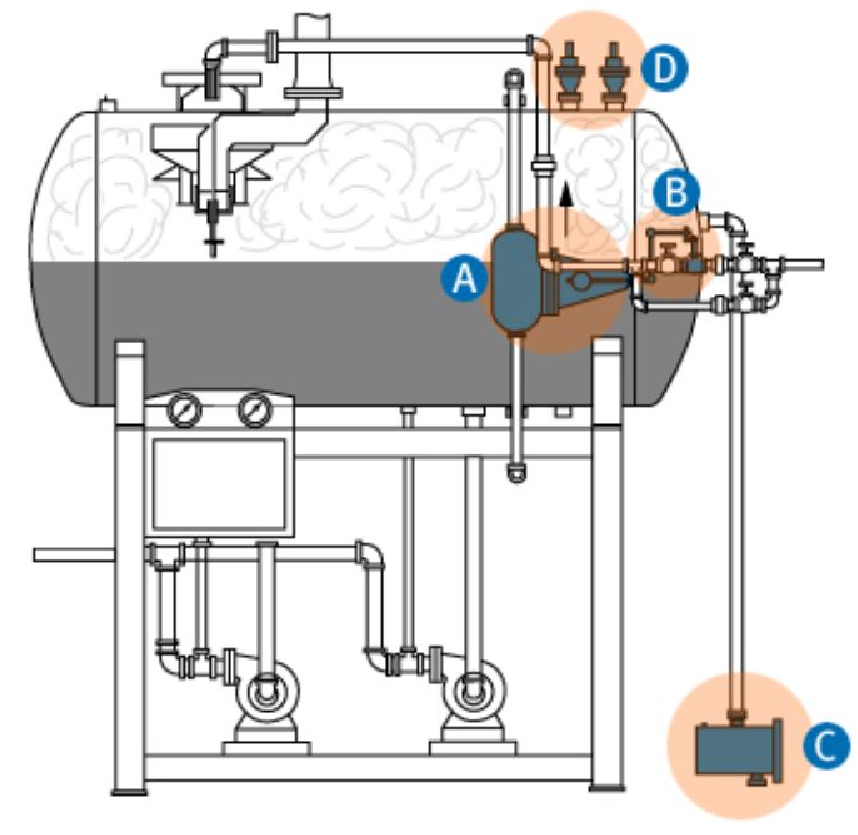
\includegraphics[width=0.5\columnwidth]{system_example.pdf}
  \caption{An example where repairing components one at a time is wasteful.}
  \label{fig:simple-example}
\end{center}
\end{figure}

To demonstrate the BRP problem, consider the system depicted in Figure~\ref{fig:simple-example}, which is a boiler tank system scheme made by Warren Controls, Inc. %ref?
When demand for water reduces the liquid level in the tank, the float cage (denoted as component $A$) opens the lever valves (component $B$) to supply intake water to the tank and closes it when the water reaches the desired level. Component $C$ is an overflow trap that collects and relieves condensate overflow. Component $D$ includes two vacuum breakers that are opened to relieve the tank with outside air to prevent vacuum pressures in the tank.

Assume some water was extracted from the tank, and so additional water is required, but we observe that the water level does not increase. There are two possible diagnoses: either the float cage $A$ is faulty or the lever valve $B$ is faulty. Assume that the probabilities of $A$ and $B$ to be faulty are given by the manufacturer and are 0.06 and 0.04, respectively. Since only these diagnoses can explain the problem, the normalized probability of $A$ to cause the problem is 0.6 and that of $B$ is 0.4. There are three possible repair actions: to repair $A$, to repair $B$, and to repair $A$ and $B$. Assume the repair cost of each component is 5\$ but the repair overhead is 50\$, due to the cost of opening the tank and boiling the water. If $A$ is repaired, there is a 0.4 chance that the system will not be fixed and another repair action will be needed (repairing $B$). Thus, the expected total repair cost of repairing $A$ first is $0.4\cdot(5+50)+5+50=77$. Similarly, the expected total repair cost for repairing $B$ first is $0.6\cdot(5+50)+5+50=88$. The best option is thus to repair $A$ and $B$ together in a single repair action, incurring an expected total repair cost of $5+5+50=60$.


%\roni{I think that we do more than modeling it as a combinatorial optimization problem. You also model it as an MDP. The paragraph below needs to be fixed to address this.} - hilla: done
In this work, we propose two approaches for solving BRP. In the first approach, we model BRP as a combinatorial optimization problem, searching in the combinatorial space of possible repair actions for the best repair action. There are two challenges in implementing this approach: (1) how to measure the quality of a repair action, and (2) how to efficiently search for the repair action that maximizes this measure. There are many efficient heuristic search algorithms in the literature, and thus we propose intelligent heuristics for estimating the merit of a repair action. In addition we cope with the second challenge by proposing greedy and optimal heuristic search and planning algorithms.
The second approach we propose for solving BRP is to model BRP as a Markov Decision Process (MDP). The main idea is 
to assess the outcome of sequences of repair actions and choosing the repair action that yields the lowest expected repair costs. 


We evaluate the effectiveness of the different BRP algorithms experimentally on two different benchmarks. The first is a standard Boolean circuit systems, which is a commonly used benchmark in the troubleshooting and diagnosis literature. The second benchmark  contains randomly generated observation from the medical physiotherapy field.
The results show clearly that that indeed considering batch repair actions can significantly save repair cost. 
Using intelligent heuristics for choosing the right batch repair action also has a crucial impact on reducing repair cost and runtime. 
%In addition, some of the algorithms mostly achieve lower cost in the expense of runtime.
%\roni{I don't think the above is really a result that we observed. Didn't hill climbing be in general awesome? re-think what you want to say here and make it consistent with your results}%%%%%%



\section{Background and Problem Definition}
%\roni{There is a bit of a mish-mash. Now you define MBD,then stop talking about it for a while and define BRP, then stop talking about BRP while and talk about diagnoses, and then talk about BRP.I recommend: say in the beginning that BRP is related to MBD. Then define MBD, diagnoses, MBDE and all that is not BRP. Only then define BRP properly.} 
%\hilla{done}
In this section, we define the batch repair problem. As a preliminary, we provide relevant background on model-based diagnosis (MBD). % and provide relevant background. %. It is important to lay the base for defining BRP, by presenting the related definitions of MBD. 

\subsection{Model-Based Diagnosis}
MBD is an approach for automated diagnosis in which a model of the diagnosed system is given and used to explain the observed abnormal system behavior. Following standard MBD terminology, we denote by $\COMPS$ and $\OBS$ the components in the system and the observed system behavior, respectively. $\SD$ describes the behavior of the diagnosed system, and in particular the behavior of each component. The term {\em behavior mode} of a component refers to a state of the component that affects its behavior. $\SD$ describes for every component one or more \emph{behavior modes}. For every component, at least one of the behavior modes must represent the normal behavior of the component. 
We denote by $\varphi_{C_i}$ the normal behavior of component $C_i$ (where $C_i\in\COMPS$). For instance, the normal behavior of the lever valve (component $B$ in Figure \ref{fig:simple-example}) is to be opened once the float cage opens it, while an abnormal behavior can be stuck open or close. $h(C_i)$ is a predicate stating that $C_i$ is healthy, i.e., in its normal mode. Formally, $h(C_i) \rightarrow \varphi_{C_i}$. 

%The normal behavior mode is often described by the clause $h(C_i) \rightarrow \varphi_{C_i}$, where $C_i\in \COMPS$. $h(C_i)$ is a predicate stating that $C_i$ is healthy, and $\varphi_{C_i}$ describes the nominal behavior of $C_i$. For instance, the nominal behavior of the lever valve (component $B$ in Figure \ref{fig:simple-example}) is to be opened once the float cage opens it, while an abnormal behavior can be stuck open or close.

A mode assignment $\omega$ is an assignment of {\em behavior modes} to components. Let $\omega^{(+)}$ be the set of components assigned their normal behavior mode and let $\omega^{(-)}$ be the set of components assigned one of the other modes.

\begin{definition}[Diagnosis]
A mode assignment $\omega$ is called a diagnosis if $\omega \wedge \OBS \wedge \SD$ is consistent.
\end{definition}

\subsubsection{An MBD Engine}


An MBD engine (MBDE) accepts as input $\SD$, $\OBS$, and $\COMPS$, and outputs a set of diagnoses $\Omega$. Note that $\Omega$ is a set since there may be more than one diagnosis, i.e., more than mode assignment that is consistent with $\SD$ and $\OBS$. 
Therefore, if there are two diagnoses, repairing the set of components in one of them may not result in the system being fixed. We say that a diagnosis $\omega$ is {\em correct} if by repairing the set of components in $\omega^{(-)}$ the system is fixed. 
Notice that according to the definition above, a diagnosis that contains all the system's components, $\omega = \COMPS$, is also considered to be {\em correct}, but of limited practical value. 

Some MBDE, return only the \emph{subset-minimal diagnoses}. A diagnosis $\omega$ is defined as a subset-minimal if there is no subset of $\omega$ that is a diagnosis. 
%which by repairing only this set of components will result with a fixed system. [[Roni: we just made the distinction between correct diagnosis and consistent, and you mean here the latter]
In our work, we use a MBDE that generates only subset-minimal diagnoses.
\roni{No need to capitalize Subset-Minimal)}

Some diagnosis algorithms return a \emph{score} for each diagnosis they return, where higher score indicates higher likelihood that the diagnosis is correct~\cite{williams2007conflict,abreu2011simultaneousDebugging}. \roni{Add a reference to Amir's 2016 paper on data-augmented software diagnosis}. Formally, let $p: \Omega \rightarrow [0,1]$ denote this likelihood score. We assume that $p(\omega)$ is normalized so that $\sum_{\omega\in\Omega} p(\omega)=1$ and use it to approximate the probability that $\omega$ is correct.


One way to obtain such likelihood scores is to assume a prior for each component on the likelihood that it has failed, denoted $p(c)$, and assume that components fail independently~\cite{Stern17shelly}. 
Under these assumptions, the likelihood score of a diagnosis can be computed as
\begin{equation}
\displaystyle p(\omega)=\frac{\prod_{c\in\omega^{-}} p(c)}{\sum_{\omega'\in\Omega}{\prod_{c\in\omega'^{-}} p(c)}}
\label{eq:likelihoods}
\end{equation}
where the denominator is a normalizing factor. 
In our experiments we computed diagnoses likelihoods computed according to Equation~\ref{eq:likelihoods}, 
but other methods for computing likelihood of diagnoses also exist~\cite{mengshoel2010probabilistic} and the algorithms we propose are agnostic to how these probabilities are found. 

\subsection{The Batch Repair Problem (BRP)}

A {\em batch repair problem} (BRP) arises exactly like a diagnosis problem: when the assumption that all components are normal is not consistent with the system description and observations. Formally,
\[ \SD \wedge \OBS \wedge \bigwedge_{C\in \COMPS} h(C) ~~~ \text{is not consistent} \]

In the example shown in Figure \ref{fig:simple-example}, assuming that all components are healthy under the observation that the water level is decreased is not consistent. Then a possible diagnosis is that components $A$, $C$ and $D$ are healthy, while $B$ is in an abnormal mode. For instance, the lever valve ($B$) is stuck close. Another possible diagnosis is that $B$, $C$ and $D$ are healthy, while $A$ is in an abnormal mode. In order to get the system to function correctly, at least one component must be repaired.

\begin{definition}[Repair Action]
A repair action can be applied to any subset of components and results in these components becoming normal. Applying a repair action to a set of components $\gamma$ is denoted by Repair($\gamma$).
\label{def:repairAction}
\end{definition}
\noindent definition ~\ref{def:repairAction} assumes that repair actions always succeed, i.e., a component is normal after it is repaired. %[Roni: TODO: discuss how to relax this assumption later in the paper.]

After a repair action, the system is tested to check if it has been fixed.
We assume that the system inputs in this test are the same as in the original observations ($\OBS$). The observed system outputs are then compared to the expected system outputs of a healthy system. Thus, the result of a repair action is either that the system is fixed, or a new observation that may help choosing future repair actions.


Repairing a set of components incurs a cost, composed of a repair overhead and component repair costs. The repair overhead is denoted by $\cost_{repair}$, and the component repair cost of a component $c\in \COMPS$ is denoted by $\cost_{c}$.
\roni{We should consider changing notation for $\cost_{repair}$ to something that indicates its only the overhead costs. Perhaps $\cost_{overhead}$ or $\cost_{oh}$}

\begin{definition}[Repair Costs]
Given a set of components $\gamma\subseteq \COMPS$, the cost of applying  Repair($\gamma$) is given by:
\[ \cost(Repair(\gamma)) = \cost_{repair} + \sum_{c\in \gamma} \cost_{c} \]
\end{definition}
We assume that all repair costs are positive and non-zero, i.e., $\cost_{repair}>0$ and $\cost_{c}>0$ for every component $c \in \COMPS$. 


%\subsubsection{The Repair Process}
%\label{sec:sysStateDuring}

To fix a system, one may need to perform more than one repair action. We use the term {\bf repair process} to refer to the process of applying these sets of repair actions until the system is fixed. The cost of a repair process is the sum of costs of its constituent repair actions. 


%That is, the cost of a repair process in which the set of performed repair actions performed is $\Gamma=(\gamma_1, \gamma_2, \ldots)$ is defined to be $\sum_{\gamma\in\Gamma} \cost(Repair(\gamma))$. 
%As defined earlier, the task in BRP is to fix a system with minimum total repair cost.\roni{Was it really defined earlier?}

\begin{definition}[BRP] 
Given $\COMPS$, $\SD$, and $\OBS$, 
The task in a BRP problem is choose actions in a repair process. 
A solution to a BRP problem is a sequence of repair actions $\Gamma=\{\gamma_1, \gamma_2, \ldots\}$ to be applied during the repair process. 
\end{definition}
The cost of a solution $\Gamma$ is the cost of the repair process that uses $\Gamma$, that is $\sum_{\gamma\in\Gamma} \cost(Repair(\gamma))$, and, of course, lower cost solutions are preferred. 
Next, we propose several algorithms for finding low-cost solutions to BRP. 
%that aim at finding a low-cost solution. 


%Obviously, lower cost solutions are preferred and  and an optimal BRP algorithm is a BRP algorithm that outputs a solution that is guaranteed to produce the so effective BRP algorithm 
.



%Therefore, an efficient BRP solver should consider the possibility of repairing a set of components in a single repair action, as shown in Figure~\ref{fig:simple-example}. Thus, the potential number of repair actions is %exponential in the number of components, in particular the power set of the components
%[[Roni: this repeats what was earlier with no new data]]
%$2^{|\COMPS|}$. Therefore, from a complexity point of view, %solving BRP via bruth force  is not feasible, even for systems of moderate size.  %is an extremely hard problem.
% NOTE: I REMOVED THE STATEMENT THAT BRP IS VERY HARD FROM A COMPLEXITY POINT OF VIEW. WE DON'T HAVE FORMAL PROOFS.
%\roni{TODO: CONTINUE FROM HERE. I THINK THE REPAIR LIKELIHOOD SHOULD GO INTO THE SOLVING PART, NOT THE DEFINITINO PART}


\section{BRP as a Sequence of Combinatorial Search Problems}

In this section, we show how BRP can be solved by reducing it to a sequence of combinatorial search problem. 
Then, we propose several heuristic algorithms for solving these combinatorial search problems.  


% System state, possible repair action
During the repair process, components are repaired and new observations are collected after every repair action. 
We use the term {\bf system state} to refer to the set of already repaired components and the set of observations collected so far, including the initial observation $OBS$. 
For a state $s$, we denote the former set by $s.\repaired$ and the latter set by $s.\observed$. 
The complement of $s.\repaired$, i.e., the set of components that were not repaired yet ($\COMPS\setminus s.\repaired$), is denoted by $s.\notrepaired$. We omit the state $s$ when it is clear from the context. 

In this work, we  assume that there is no need to repair a component twice in the same repair process. Thus, $2^{s.\notrepaired}$ represents all possible (single or batch) repair actions needed to fix the system from state $s$, where $2^{s.\notrepaired}$ is the power set of $s.\notrepaired{}$. 
A solution to BRP can therefore be obtained by choosing a repair action from 
$s.\notrepaired{}$ in every reached system state $s$, performing the chosen action, and repeating the process 
until the system is fixed. 

The \emph{search-based approach} for solving BRP is to choose a repair action in a system state $s$
but defining a utility function that estimates the merit of repair actions and then find the repair action that maximize this utility. The challenge in this approach is two-fold: how to estimate the utility of a repair action, 
and how to find the repair action that maximizes this utility in the combinatorial space of $2^{s.\notrepaired}$  actions. Next, we describe how we addressed these challenges.


\subsection{BRP Utility Functions} 
%As explained above, the search problem comes down to finding the repair action that maximizes a utility evaluation function $U(\cdot)$ that maps a repair action to a real value that estimates its merit. 
%\subsubsection{k-Highest Probability}

A key source of information for all the utility functions described below is the set of diagnoses $\Omega$ and their likelihoods ($p(\cdot)$). 
%We assume that this information is obtained by using a diagnosis engine over the observations of the current state of the system. The set of returned diagnoses may be very large. 
The first utility function we propose is based on the system's {\em health state}, which has been recently proposed as a method for aggregating information from a set of diagnoses~\cite{Stern17shelly}.

\begin{definition}[Health State]
A health state is a mapping $F: COMPS\rightarrow [0,1]$ where
\[ \displaystyle F(C)=\sum_{\omega\in \Omega s.t. C\in \omega} p(\omega)\]
\label{def:health-state}
\end{definition}
$F(C)$ is an estimate of the likelihood that component $C$ is faulty given a set of diagnoses $\Omega$ and their likelihoods.
Based on the system's health state, we propose the following utility function, denoted $U_{HP}$:
\[
U_{HP}(\gamma) = \sum_{C\in \gamma} F(C)
\]
where $\gamma$ is a subset of $COMPS$ that were not repaired yet.


The repair action that maximizes $U_{HP}$ is trivial --- repair all components.
This would result in the system being repaired, but of course, may repair many components that are likely to be healthy. To mitigate this effect, we propose the {\em $k$ highest probability} utility function, 
which assigns zero utility for repair actions
that consists repairing more than $k$ components, where $k$ is a user-defined parameter. 
In effect, using this utility means limiting the number of components that can be repaired in a single repair action to $k$. 

Finding the batch repair action that maximizes this utility function does not require any exhaustive search: simply sort the health state in descending order of $F(\cdot)$ values and repair the first $k$ components. We call the resulting BRP algorithm the $k$-HP repair algorithm. 


Although the $k$-HP repair algorithm is computational light, it has two clear disadvantages. First, the user needs to define $k$. Second, $k$-HP does not consider repair costs (neither component repair costs nor overhead costs).
%MEIR: i did not understand the last sentence.
The next set of utility functions address these disadvantages.

\subsubsection{Wasted Costs Utilities}

%Repairing a system requires performing repair actions.
Some repair costs are inevitable: the component repair costs for the faulty components
and the repair overhead of a single repair action. We propose a family of utility functions that try to estimate the expected total repair costs beyond these inevitable costs. We refer to these costs as {\em wasted costs} and to utility functions of this family as {\em wasted cost functions}. We model these wasted costs as being composed of two parts.
\begin{itemize}
\item {\bf False positive costs ($cost_{FP}$).} These are the costs incurred by repairing components that are not really faulty.
\item {\bf False negative costs ($cost_{FN}$).} These are the overhead costs incurred by future repair actions.
\end{itemize}




%\meir{I think this para is redundant, since the para after it explains the same clearer.} It is clear why the false positive costs are wasted costs --- these are repair costs incurred on repairing healthy components. The false negative costs are wasted costs because if one knew upfront which components are faulty, then the optimal repair algorithm would repair all these components in a single batch repair action, incurring no further overhead costs. Thus, future overhead costs represent wasted costs.


We borrow the terminology of false positive and false negative from the machine learning literature, but use it in a somewhat different manner. To explain this choice of terminology, assume that positive and negative mean faulty and healthy components respectively. Choosing to repair a faulty component is regarded as a true positive, and not repairing a healthy component is regarded as a true negative. Thus, the wasted costs incurred by repairing healthy components are costs incurred due to false positives, and the wasted costs incurred by not repairing a faulty component are overhead costs incurred due to false negatives. While this is not a perfect match in terminology, we believe that it helps clarify the underlying intention of $cost_{FP}$ and $cost_{FN}$.





%$2^{|\COMPS|}$. Therefore, from a complexity point of view, %solving BRP via bruth force  is not feasible, even for systems of moderate size.  %is an extremely hard problem.



%moved the following text (used to be under search algorithms) up to here as we discussed ------------
%As noted earlier, finding the best batch repair action according to the $k$-HP utility function is easy. 
%This is not the case when using as a utility function one of the functions from the wasted effort family. 


%fix- costFN and costFP have not been defined yet
%\begin{definition}[Minimal BRP Wasted Cost Problem]
%Given a BRP problem and a definition of $cost_{FN}$ and $cost_{FP}$, the minimal BRP wasted cost problem, denoted \brps{} is the problem of 
%finding a subset of components $\gamma$ that minimizes $C_{WC}$. 
%\end{definition}
%Clearly, an optimal solution to \brps{} is a repair action that maximizes $U_{WC}$, since the goal is to minimize $C_{WC}$ and $U_{WC} = - C_{WC}$, as defined earlier .


\noindent \textbf{The Wasted Cost Utility Function.}
For a given set of components $\gamma$, we denote by $cost_{FP}(\gamma)$ and $cost_{FN}(\gamma)$ the false positive costs and false negative costs, respectively, incurred by performing a batch repair action of repairing all the components in $\gamma$. In addition, we denote by $\sysrep{\gamma}$ the probability that the system is fixed after the components in $\gamma$ are repaired. 



Given $cost_{FP}(\gamma)$, $cost_{FN}(\gamma)$, and $\sysrep{\gamma}$, we propose the following general formula for computing the expected wasted costs, denoted by $C_{WC}$.
\begin{equation}
C_{WC}(\gamma)=cost_{FP}(\gamma)+(1-\sysrep{\gamma})\cdot cost_{FN}(\gamma)
\label{eq:wc}
\end{equation}
The left hand side of the formula is the false positive costs. The right hand side of the formula is the false negative costs, multiplied by the probability that the system will not be fixed by repairing the components in $\gamma$. Thus, the formula gives the total expected wasted costs.
We define $U_{WC}(\gamma)=-C_{WC}(\gamma)$ as the {\em wasted cost utility function}.


%Clearly, an optimal solution to \brps{} is a repair action that maximizes $U_{WC}$, since the goal is to minimize $C_{WC}$ and $U_{WC} = - C_{WC}$, as defined earlier .

%BRPswc is NP-hard:
%We claim that \brpswc{} is NP-hard. In order to prove so, we will demonstrate how a solution for Minimal Hitting Set can be found by solving \brpswc{}. The input of the Minimal Hitting Set problem is a group of n groups of entities, ${\gamma_1,...,\gamma_n}$, and represent the possible repair actions for \brpswc{}. The entities in the groups, which represents a component in \brpswc{}, defined with an equal prior probability to be faulty, p. Furthermore, the $cost_{FN}$ and $cost_{FP}$ defined as follow: ${cost}_{FP}(\gamma) = |\gamma|$${cost}_{FN}(\gamma) = 1/n$


The wasted cost utility function is a theoretical utility function, since one does not know upfront the values of $cost_{FP}$ and $cost_{FN}$. Next, we propose several ways to estimate $U_{WC}$ by showing how to compute $\sysrep{}$ and proposing several ways to estimate $cost_{FP}$ and $cost_{FN}$.



\noindent \textbf{Computing the System Repair Likelihood ($\sysrep{}$).}

%\subsubsection{System Repair Likelihood}\label{sec:Repair_Likelihood}
%If the MBDE returns a single diagnosis $\omega$ that is guaranteed to be correct, then the optimal solution to BRP would be to perform a single repair action: Repair($\omega^{-})$. 
%This, however, is rarely the case, and more often a possibly very large set of diagnoses is returned by diagnosis algorithms. This introduces uncertainty in whether a repair action would actually fix the system. %We define this uncertainty as follows: I dont' get this sentence
%\begin{definition}[System Repair Likelihood]
%The System Repair Likelihood of a set of components $\gamma\subseteq \COMPS$, denoted \sysrep{$\gamma$}, is the probability that Repair($\gamma$) will fix the system.
%\end{definition}

Consider the relation between $p(\omega)$ and \sysrep{$\omega$}. If $\omega$ is correct, then repairing all components that are faulty, meaning $\omega^{(-)}$, will fix the system. Therefore, the likelihood of repairing $\omega^{(-)}$ causing the system to be fixed is at least $p(\omega)$, i.e.,
\[ \sysrep{\omega^{(-)}}\geq p(\omega)  \]
Moreover, if $\omega$ is correct then repairing any superset of $\omega^{(-)}$ would also fix the system. Thus, $\sysrep{\omega^{(-)}}$ may be larger than $p(\omega)$.
On the other hand, repairing any set of components that is not a superset of $\omega^{(-)}$, wll not fix the system, as there would still be faulty components that were not repaired. 
Therefore, a repair action Repair($\COMPS '$) would fix the system if and only if $\omega^{*{(-)}}\subseteq \COMPS '$, where $\omega^*$ is the correct diagnosis.
While we do not know $\omega^*$, we can compute \sysrep{$\gamma$} from $\Omega$ and $p(\cdot)$:
\[ \sysrep{\gamma} = \sum_{\omega\in \Omega \wedge \omega\subseteq \gamma} p(\omega) \]
\sloppy{For example, in the boiler tank depicted in Figure~\ref{fig:simple-example}, there are two diagnoses, $\{A\}$ and $\{B\}$, such that $p(\{A\})=0.6$ and $p(\{B\})=0.4$. Thus, $\sysrep{\{A\}}$=0.6, $\sysrep{\{B\}}$=0.4, and $\sysrep{\{A,B\}}$=$p(\{A\})$+$p(\{B\})$=1.}


\noindent \textbf{Estimating the False Positives Cost.}
We propose to estimate the false positive costs by considering the system's health state (Definition~\ref{def:health-state}), as follows.

\[ \widehat{cost}_{FP}(\gamma)=\sum_{C\in \gamma} (1-F(C))\cdot cost(C) \]
This estimate of the false positive costs can be understood as an expectation over the false positive costs. The cost of a repaired component $C\in\gamma$ is part of the false positive costs only if $C$ is in fact healthy. The probability of this occurring is $(1-F(C))$. Thus, $(1-F(C))\cdot cost(C)$ is the expected false positive cost due to repairing component $C$.

\noindent \textbf{Estimating the False Negatives Cost.}
Correctly estimating $cost_{FN}$ is more problematic than $cost_{FP}$, as it requires considering the future actions of the repair algorithm.
In the best case, only one additional repair action would be needed. This would incur a single additional overhead cost. We call this {\bf the optimistic $cost_{FN}$}, or simply $cost_{FN}^o$, which is equal to $cost_{repair}$.
The other extreme assumes that every component not repaired so far would be repaired by a single repair action, and correspondingly an incurred overhead cost. We experimented with a slightly less extreme estimate, in which we assume that only faulty components will be repaired in the future, but each will be repaired in a single repair action, incurring one $cost_{repair}$ per faulty component.
Since we do not know the number of faulty components, we use the expected number of faulty components according to the health state: $\sum_{c\notin \gamma} F(c)$. The resulting estimate is referred to as {\bf the pessimistic $cost_{FN}$}, denoted by $cost_{FN}^p$, is thus computed as:
\[ cost_{FN}^p(\gamma)=cost_{repair}\cdot \sum_{c\notin \gamma} F(c)\]

\noindent \textbf{Enhanced Wasted Cost Utility Function.}
An important computational inaccuracy is taking place on the computation of $cost_{FN}^p$ as described above. To explain that, first we need to better understand the computational meaning of changing the state of the system. We denote the $system state$ resulted from repairing a set of components $\gamma$ by $sysState(\gamma)$. Assuming that the system is not fixed after repairing a set of components $\gamma$, there will be new set of diagnoses in correspondence to $sysState(\gamma)$ (see Section~\ref{sec:sysStateDuring}).
The change in the diagnoses effects the health state of each components, $F(c)$, and as a result the false negative costs estimation could be effected as well. As described, the pessimistic estimation of $cost_{FN}$ aspires to compute the future repair costs of components that has not been fixed, while using the health state to estimate the probability of each component to be faulty. However, those estimated probabilities derived from the current $system state$ instead of the next $system state$, which is the resulted state after executing the repair action. Meaning, the used health state in the computation of $cost_{FN}^p$ could be in-accurate, relatively to the next system state.
As a result, we propose another alternative estimation for the $cost_{FN}$:
\[ cost_{FN}^{{{p}'}}(sysState(\gamma))=cost_{repair}\cdot \sum_{c\in \overline{Repaired} \in sysState(\gamma)} F(c)\]

Notice that all of the described $cost_{FN}$ estimation up to this point computes the future costs under a naive assumption; Only faulty components will be repaired in the future. There is no explicit consideration of the future false positive costs, i.e., the cost that will be wasted in the future when repairing components that should not have been repaired. 
To account for the future false positive costs, we add the same computation computed for the current false positive costs, but over all the components not chosen by the current repair action. 
Thus, for a batch of components $\gamma$, we estimate the future false positive costs, denoted $cost_{FFP}(\gamma)$, as follows:
\[
cost_{FFP}(sysState(\gamma))=\sum_{c\in \overline{Repaired} \in sysState(\gamma)} (1-F(c))\cdot cost(c) 
\] 
The resulting wasted cost utility function, which we refer to as ``pessimistic FFP enhanced'',  is given by:
\begin{multline}
C_{WC}(\gamma)=cost_{FP}(\gamma)+(1-\sysrep{\gamma}) \cdot \\ (cost_{FN}^{{{p}'}}(sysState(\gamma))+ cost_{FFP}(sysState(\gamma)))
\end{multline}

In general, this reasoning can be taken even further; A possible development of the pessimistic FFP enhanced could be to deepen the assessment of future repair actions and estimated future wasted cost. In other words, a good utility function which aspires to provide an assessment to the future wasted costs after performing a repair action, could achieve it by performing a recursive (or pseudo-recursive) process, such that the future wasted costs of a repair action $(\gamma)$ would be the average future wasted costs of each possible repair action that could be taken in $sysState(\gamma)$. Formally:
$futureWC(\gamma) = average_{\gamma{}'\subseteq \overline{Repaired} \in sysState(\gamma)}(futureWC(\gamma{}'))$

To summarize, we presented three variations of the wasted cost utility function, which all present two factors that affect the corresponding version of the utility function: (1) false positive cost, and (2) two alternatives of false negative cost (optimistic and pessimistic), and only in one version there is an additional consideration in the future false positive cost.


We observed experimentally (see Section~\ref{sec:experimental-results} that choosing repair actions according to the wasted cost utility function is effective in reducing the overall cost of the repair process. However, finding the best repair action according to the wasted cost utility function, is a non-trivial combinatorial search problem. 
\begin{definition}[Minimal BRP Wasted Cost Problem]
For a given BRP instance and an expected wasted cost function $C_{WC}$, 
the minimal BRP wasted cost problem is the problem of 
finding a subset of components $\gamma$ that minimizes $C_{WC}$. 
\end{definition}
Next, we discuss several combinatorial search frameworks for solving the \brpswc{}.

%TODO: prove that its NP hard-------------------------------------------

\subsection{Search Space Formulation}

\begin{figure}
\centering
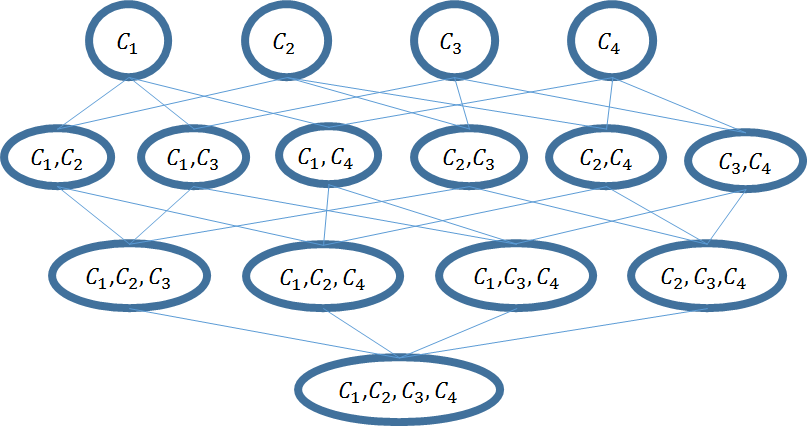
\includegraphics[width=0.75\columnwidth]{PowersetBasedSearch.png}
\caption{An example of a powerset-Based search space }
\label{fig:power-search-space}
\end{figure}

\begin{figure}
\centering
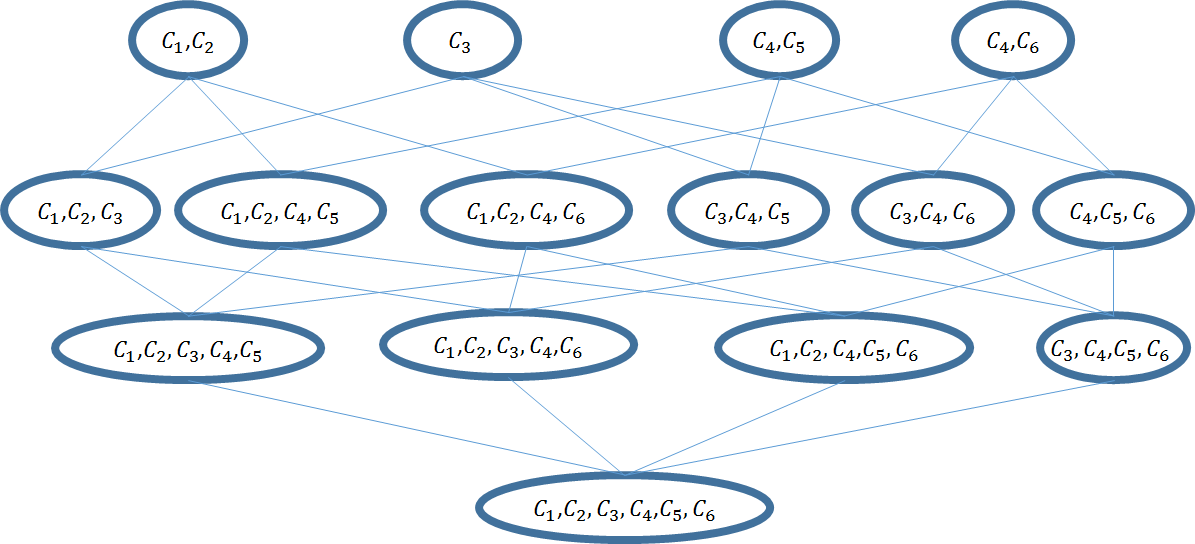
\includegraphics[width=0.85\columnwidth]{UnionBasedSearch.png}
\caption{An example of a union-based search space}%
\label{fig:union-search-space}
\end{figure}

The first step in solving a combinatorial search problem is to define its search space. 
For \brpswc{}, a natural way to defines the search space is as a lattice of all possible subsets of components that were not repaired so far. A state $s$ in the search space defines as a set of components, denoted $\comps[s]\subseteq\notrepaired{}$. 
A state transition from $s$ represents adding a single component to $\comps[s]$. 
The initial state, i.e., the root of the search space, is an empty set. %superset of $\gamma$ in which  to be repaired in a single batch repair action. A Furthermore, an edge from node $V$ to ${V}'$, which defined by $\gamma$ and ${\gamma}'$ respectively, indicates that ${\gamma}'\subset\gamma$. 
%\begin{definition}[BRP as a search problem] Node $V$ defined as a subset of components $\gamma \subset COMPS$ to be repaired in a single batch repair action, where $\gamma$ is a subset of $COMPS$ that were not repaired yet. Edge $E$ represented by the pair $(V,{V}')$, if ${V}'$ is a direct child node of $V$ in the search space. Furthermore, an edge from node $V$ to ${V}'$, which defined by $\gamma$ and ${\gamma}'$ respectively, indicates that ${\gamma}'\subset\gamma$.  \end{definition} 
 	Figure~\ref{fig:power-search-space} illustrates this search space for a system with four components, $C_1, C_2, C_3,$ and $C_4$. We call this search space formulation the {\em powerset-based search space}. 
	
	
	An alternative approach, which we refer to as the {\em union-based search space}, 
	is to consider the set of diagnosis $\Omega$ obtained by MBDE, 
	and limit the search space to all possible unions of diagnoses from $\Omega$. In this search space the root of the search is still an empty set of components, but its children are all subsets of components that form a diagnosis. The $i^{th}$ level of the search space consists all subsets of components that are unions of $i$ diagnoses from $\Omega$.  Figure~\ref{fig:union-search-space} illustrated an example of this union-based search space space, for a system with six potential faulty components, $C_1, C_2, C_3, C_4, C_5$ and $C_6$, where the MBDE outputted four diagnoses $\Omega=\{\left \{C_1, C_2\}, \{C_3\}, 
	\{C_4, C_5\}, \{C_4, C_6\}\right\}$. The root of the search space is omitted. 
	%were the given set of four diagnoses are represented by the nodes in the first level of the search tree.
	
The idea behind this approach has an intuitive reasoning that according to the known observation at least one of the diagnosis in $\Omega$ is supposed to be true. Thus, a repair action that does not repair all the components in at least one diagnosis cannot result in a fixed system. For example, if we look at the diagnoses of the case depicted in Figure~\ref{fig:union-search-space}; $\omega_1={C_1,C_2}$, $\omega_2={C_3}$, $\omega_3={C_4,C_5}$, $\omega_4={C_4,C_6}$. If the chosen repair action would have been for instance ${C_1}$, the system would not be fixed after repairing that component, and at least one more iteration of diagnosis, repair and testing would have to take place. That would be resulted with potentially higher total repair costs due to the $\cost_{repair}$.


To summarize the differences of the two presented search space formulations, in the {\em powerset-based search space}, the children of a state representing a repair action $\gamma$ are all the sets of components that can be created by adding a single component to $\gamma$. In {\em union-based search space}, the children of a state are all sets of components that can be created by adding the components from a single diagnosis to $\gamma$. %We compare these search space formulations experimentally in Section~\ref{sec:experimental-results}.


\subsubsection{Search Space Properties}
\label{sec:search-space properties}
Both search space spaces -- powerset-based and union-based -- can be very large even for medium sized systems with hundreds of components. 
The worst-case branching factor is $|\COMPS|$ and $|\Omega|$ for the powerset-based and union-based search space, respectively. 
The number of states in the search space is $|2^{\COMPS}|$ and $|2^{\Omega}|$ for the powerset-based and union-based search space, respectively. 

Which search space is larger depend on how $\Omega$ is structured, i.e., in the output of the MBDE. 
If the MBDE outputted a small number of diagnoses, then the union-based search space may be much smaller than the powerset-based one, 
especially the diagnoses contain multiple components. In the extreme case, the MBDE outputs a single diagnosis, in which case 
the union-based search space will have a single state regardless of how many components are in that diagnosis. 

However, the number of diagnoses an MBDE may return can be exponential in the number of components, as every subset of components may, in theory, be a diagnosis. 
In some standard MBD benchmarks, systems with several thousands of component have over a million subset-minimal diagnoses~\cite{Stern17shelly}. 
Thus, the worst-case size of the union-based search space is $2^{2^{|\COMPS|}}$, much more than the worst-case size of the powerset-based search space, which is $2^{|\COMPS|}$. 
In our experiments (Section~\ref{sec:experimental-results}), we implemented both search space formulations and compared the performance of search algorithms that use them. 



\subsection{Search Algorithms}

Given an objective function and a search space, 
the missing part for solving \brpswc{} is a search strategy. We propose two baseline search strategies, breadth-first search (BFS) and Hill Climbing, and a more sophisticated method based on the A* algorithm~\cite{hart1968formal}. 

%As a baseline, we propose two simple search strategies. 

%-----------
%\subsubsection{Uninformed Search}
\subsubsection{Baseline Strategies}

In first baseline search strategy, BFS, 
the search explores the search space in a breath-first manner and returns the state -- a repair action -- with the lowest $C_{WC}$. 
To make the runtime manageable, we limit the depth of the BFS to a pre-defined depth-limit parameter $k$. That is, the search will explore the first $k$ levels of the search space, and return the best repair action found in these levels. 


In the second baseline strategy, Hill Climbing, 
the search explore the search space in a greedy manner, starting from the root (representing an empty repair action) and moving in every iteration to the most promising child, as measured by the lowest $C_{WC}$. The search halts when reaching a state that is a local minimum, i.e., that all its children have higher $C_{WC}$. 


We acknowledge that Hill Climbing is a very simple search search algorithm, and there are many other, more sophisticated, local search algorithms that can be used.  Techniques such as random restarts, simulated annealing, Tabu search~\cite{glover2013tabu}, and others have been shown to be very effective in many domains. However, non of these techniques can guarantee that the found repair action is indeed optimal. Next, we propose a search algorithm for \brpswc{} that is guaranteed to return an optimal solution. %can provide such guarantees. 
%~\cite{lourencco2003iterated}


%effort that is smaller we compute the expected wasted effort of every child of the root and choose the child that minimizes it. Then, we compute the expected wasted effort of every child of the chosen state and again choose the child with the lowest expected wasted effort. This process continues as long as there is a child whose expected wasted effort of the current state  the children of that state process then repeats with this chosen child, checking all its children and choosing the one with the minimal expected wasted effort. check every child of root and  , where we start from the root of the search space and in every iteration we choose to expand  the most promising child of the current state adding the components in one action to the batch repair action. All possible components are considered, and the wasted cost of the resulting batch repair action is computed.  If there exists a set of components that can be added and that will result in decreasing the wasted cost, then the one that decreases the wasted cost the most is chosen. Otherwise, the current batch repair action is returned. [[Roni: this is confusing with the subset and union-based difference]


\subsubsection{Optimal Search}


One of the most well-known optimal search algorithms is \astar{}~\cite{hart1968formal}. \astar{} follows a best-first search algorithmic framework. It maintains a list of open nodes (denoted OPEN), initialized by the root of the search tree. 
In every iteration it pops from OPEN the node $n$ with the lowest $f(n)=g(n)+h(n)$ value, where $g(n)$ is the cost spent so far for node $n$, and $h(n)$ is an estimate of the lowest cost path from $n$ to a goal. Then, $n$ is {\em expanded}, which means that all its children (the nodes created by applying a single state-transition operator on $n$) are {\em generated} and inserted to OPEN. If the heuristic $h(n)$ is \emph{admissible}, which means it is a lower bound to the lowest-cost path from $n$ to a goal, then, under certain conditions, \astar{} is guaranteed to have found an optimal solution once a goal has been expanded~\cite{hart1968formal}. 

% Challenges in A*
Applying textbook \astar{} to solve \brpswc{} is non-trivial due to several reasons. First, in \brpswc{} every state is a goal state, as every state represents a possible batch repair action. Clearly, expanding only the root of the search tree is not sufficient to guarantee optimality. 
Second, to solve the \brpswc{} problem with \astar{}, one needs to define $g(n)$ and $h(n)$, which are both costs associated with a \emph{path} (from start to $n$ and from $n$ to a goal). However, in \brpswc{} a \emph{path} in the search space has no real notion of cost. That is, a  \emph{state} in \brpswc{} has a cost -- its expected wasted costs $C_{WC}$ -- but what is the cost of a path?

% From path-based A* to state-based
To move from a path-based \astar{} to a state-based \astar{}, we considered the following state-based values:
\begin{itemize}
    \item \textbf{$cost(n)$.} The expected wasted costs of $\comps[n]$, i.e., $C_{WC}(\comps[n])$.
    \item \textbf{$L(n)$.} A heuristic function that estimates the cost of the lowest cost node in the subtree of the \brpswc{} search space rooted at $n$ (including $n$). 
\end{itemize}
We say that $L(n)$ is admissible if is a lower bound on the value it estimates: \begin{equation}
 L(n)\leq \min \{cost(n')| \comps[n] \subseteq \comps[n'] \}  \label{eq:admissibility}
\end{equation}
The relation to the $g(n)$ and $h(n)$ from the textbook A* is straightforward: $cost(n)=g(n)$ and $L(n)=f(n)=g(n)+h(n)$. Similarly, if $L(n)$ is admissible then $h(n)$ is and vice-versa. However, it is more convenient in state-based problems such as \brpswc{} to discuss costs and heuristics in terms of costs and heuristics over states, instead of paths.


% The concrete algorithm
Running \astar{} with $cost(n)$ and an admissible $L(n)$ is done as follows. In every iteration the node with the minimal $L(n)$ is expanded. 
If $cost(n)$ is smaller than the incumbent solution, i.e., the lowest-cost solution found so far, then the incumbent solution is updated. The search continues until 
the cost of the incumbent solution is lower than or equal to the minimal $L(n)$ in OPEN. 

% Optimality
Note that unlike textbook \astar{}, expanding the first goal found is not a sufficient condition for guaranteeing optimality, because this search space is not monotone~\cite{stern2014max}. However, when the cost of the incumbent solution is lower than or equal to $L(n)$, then we are guaranteed to have found the repair action with the lowest expected wasted costs. To see this, 
observe that the minimal $L(n)$ in OPEN is a lower bound on the optimal solution. 
Thus, if we have an incumbent solution that is lower than or equal to the minimal $L(n)$ then it must be optimal.  
% Relation to textbook A*






\subsubsection*{Admissible Heuristics for \brpswc{}}
Next, we present several admissible heuristics for \brpswc{}, based on the structure of the wasted cost functions. 

Let $S(\gamma)$ denote the set of all supersets of $\gamma$, and let $S_i(\gamma)$ be a subset of $S(\gamma)$ consisting all supersets of $\gamma$ that have exactly $|\gamma|+i$  components. From the search space perspective, 
for a node $n$ in the search tree, $S(\comps[n])$ consists all the batch repair actions represented by nodes in the subtree rooted by $n$, and $S_i(\comps[n])$ consists all batch repair actions represented by states in the $i^{th}$ level of the subtree rooted by $n$. 


We construct an admissible heuristic function for \brpswc{} in two stages. First, we  propose a function $L(n,i)$ that bounds the cost of all states in $S_i(\comps[n])$. We call such functions an {\em $i$-level admissible} heuristic function. Given an $i$-level admissible heuristic $L(i,n)$, we construct $L(n)$ by choosing the minimum over every value of $i$. The maximal number of levels under node $n$ in the search spaceis $|\notrepaired{}\setminus\comps[n]|$ and we denote it by $m_n$.  
Formally, $L(n)$ is defined as follows:
\begin{equation}
L(n)=\min_{i=[1,\ldots, m_n]} L(n,i)
\label{eq:b-admissible}
\end{equation}

Note that for a bounded A* search, where the search is limited to a given depth, the maximal number of levels under node $n$ is determined according to the given bound.
\roni{This is out of context here as no one knows at this stage what is bounded A* serach. TODO: MOVE TO THE EXPERIMENTAL RESULTS}

\subsubsection*{i-Level Admissible Heuristics}

All the proposed expected wasted costs functions follow the framework given in Equation~\ref{eq:wc}. That is, the consists of using 
an estimate of false positive costs ($cost_{FP}(n)$), 
the system repair likelihood ($\sysrep(\comps[n])$), 
and an estimate of the false negative costs ($cost_{FN}(n)$). 
We propose an $i$-level admissible heuristic that bounds each of these components according to how they are used in Equation~\ref{eq:wc}. That is, we compute a lower bound on $cost_{FP}$, an upper bound on $\sysrep(\comps[n])$, 
and a lower bound on $cost_{FN}$. 


\noindent {\bf Bounding the false positive cost.} 
Let $C_1,\ldots, C_{m_n}$ be the list of all the components in $\notrepaired{}\setminus\comps[n]$, sorted in ascending order according to the product of the probability that they are faulty and the cost of repairing them. I.e., for every $i<j$, 
$F(C_i)\cdot cost(C_i)\leq F(C_j)\cdot cost(C_j)$. 
For every $i\in [1,m_n]$, the sum $L_{FP}(n)=\sum_{j=1}^i F(C_i)\cdot cost (C_i)$ is a lower bound  on the false positive costs added to $cost(n)$ by any repair action in $S_i(\gamma)$.
Formally, for every $n'$ in the subtree beneath $n$ (i.e., $\forall n'\in S_i(\comps[n])$), it holds that
\begin{equation}
cost_{FP}(\comps[n])+ L_{FP}(n) \leq cost_{FP}(\comps[n'])
\label{eq:fp-bound}
\end{equation}


\noindent {\bf Bounding the system repair likelihood.}
To bound the system repair likelihood, we approximate for every component how much adding it to the current repair action will increase the system repair likelihood ($\sysrep(\comps[n])$). Let  $\Omega_{\hat{n}}$ the set of diagnoses that are not equal to or a subset of $\comps[n]$. If either of these diagnoses is correct then the system will not be repaired by the batch repair represented by $n$. 
We compute for every component $C$ that is not in $\comps[n]$ but is part of a  diagnosis in $\Omega_{\hat{n}}$ the sum of the probabilities of diagnoses in $\Omega_{\hat{n}}$ that contain it, i.e,. 
\( \sum_{\omega\in \Omega_{\hat{n}}\wedge C\in \omega} p(\omega) \), 
and denote this value by $p(C)$. Clearly, adding $C$ to the repair action defined by $n$ will not increase the system repair likelihood by more than $p(C)$. 
Let $p_1, \ldots p_{m_n}$ be the list of $p$-values for every component in 
$\notrepaired{}\setminus\comps[n]$, sorted in descending order. I.e., $p_1\geq p_2, \ldots \geq p_{m_n}$. 
Finally, we define $U_{\sysrep{}}(n)=min(1, \sum_{j=1}^i p_i)$, which is an upper bound on the increase to $\sysrep{\comps[n]}$ that can be achieved by adding $i$ more components to $\comps[n]$. That is, for every $n'\in S_i(\comps[n])$, it holds that:
\begin{equation}
\sysrep{\comps[n]}+\\ U_{\sysrep{}}(n) 
 \geq  \sysrep{\comps[n']}
\label{eq:sysrep-bound}    
\end{equation}


\noindent {\bf Bounding the false negative costs.}
Bounding the false negative costs depend on the expected wasted costs function used. 
% \brpswc{} variant. 
For the optimistic case, the false negative cost are always $cost_{repair}$. 
For the pessimistic case, we take a similar approach to that used to estimate the false positive costs: sort components in ascending order according to their $F(c)$ values and take the sum of the first $i^{th}$ components. Following the same reasoning as explained for bounding the false positive costs, this too is a lower bound on false negative costs added by in any node under $n$ over the false negative costs of $n$. 
Let $L^o_{FN}(n)$ and $L^p_{FN}(n)$ be the resulting lower bounds for the optimistic and pessimistic estimates of the false negative costs, respectively. We omit the superscript (``o'' or ``p'') when it is not needed for exposition. 


Finally, we can define our $i$-level admissible heuristic as the combination of all three bounds, corresponding to Equation~\ref{eq:wc}:
\begin{multline}
    L(n,i)=\left(cost_{FP}(\comps[n])+ L_{FP}(n)\right)+\\
    \left(1-(\sysrep{\comps[n]}+ U_{\sysrep{}}(n))\right)\cdot \\
    \left(cost_{FN}(\comps[n])+ L_{FN}(n)\right)
    \label{eq:i-level}
\end{multline}
The admissibility of this $i$-level heuristic follows direction from 
Equations~\ref{eq:wc},~\ref{eq:fp-bound}, and~\ref{eq:sysrep-bound}. 
    

%\begin{equation}
%C_{WC}(\gamma)=cost_{FP}(\gamma)+(1-\sysrep{\gamma})\cdot cost_{FN}(\gamma)
%\label{eq:wc}
%\end{equation}

%C_{WC}(\gamma)=cost_{FP}(\gamma)+(1-\sysrep{\gamma})\cdot cost_{FN}(\gamma)Let $n'$ be a state in the subtree rooted by $n$. Thus, $\comps[n]\subset\comps[n']$. 


%In order to ensure admissibility we offer an alternation for the presented $i$-level admissible heuristic, i.e., $L(n,i)=b(n)+(-U_{\sysrep{}}(n))\cdot(L_{fn}-L_{fp})$. The alternative heuristic forgoes the additional false positive costs that could be added as a result of adding more components to the repair action. This change has been implicated in order to avoid double consideration in the false positive costs, thus, the false negative costs includes estimation of future repair actions. Furthermore, adding a component to the current repair action should be resulted with a change in the estimation of the false negative costs, thus that an additional component should not be considered as a future repair action and its costs need to be deducted from the false negative costs. That is the reason for subtracting the $L_{fp}$ from $L_{fn}$ in the alternative heuristic. It is easy to see that $b_L(n,i)$ is an $i$-level admissible heuristic, and consequently the $b_L$ heuristic given in Equation~\ref{eq:b-admissible} is admissible. [[Roni: all this does not make sense to me and should simply be a formal proof]]
%prove?

%bounded fval


%We acknowledge that Hill Climbing is a very simple local search search algorithm, and there are many other, more sophisticated, local search algorithms~\cite{lourencco2003iterated} that can be used.  Techniques such as random restarts, simulated annealing, Tabu search~\cite{glover2013tabu}, and others have been shown to be very effective in many domains. 

%The admissible heuristic given
There are more sophisticated optimal heuristic search algorithm beyond \astar{}, such as Enhanced Partial Expansion A*~\cite{goldenberg2014enanced}, IDA*~\cite{korf1985depth}, and RBFS~\cite{korf1993linear}, as well as a variety of bounded suboptimal search algorithms. However, the goal of this work is not to perform a comprehensive comparison of different search paradigms, but to demonstrate their potential use in solving BRP.

\section{BRP as a Planning Problem}
The second approach we propose for solving BRP, models it as a Stochastic Shortest Path Markov Decision Process (SSP-MDP)~(\cite{bertsekas1995dynamic}). An SSP-MDP is a common model for planning problems where actions may have stochastic outcomes, and the task is to reach a goal state with minimal expected cost. 
In BRP, repair actions have stochastic outcomes -- the system is either fixed or not -- and our aim is to minimize the expected repair costs incurred until the system is fixed. 
 %Following the maximum expected utility principle, we aim at

Formally, an SSP-MDP is defined by a tuple $\left \langle S, A,Tr,R,I,G \right \rangle$ where $S$ and $A$ are the sets of states and actions respectively. $Tr(s,a,{s}')$ is the transition function, returning the probability that performing action $a$ at state $s$ leads to state ${s}'$. $R(s,a)$ is the reward of performing an action $a$ at state $s$. $I$ is the initial states and $G$ is the set of terminal states.

In our case, states are the \emph{system states} during a repair process and actions are the \emph{repair actions}. The reward of performing a repair action $\gamma$ is minus the cost of the corresponding repair action, $-cost(Repair(\gamma))$. The possible outcomes of an action are that the system is fixed or not. The probability of each outcome is given by \sysrep{}. An outcome where the system is fixed corresponds to a goal state. Otherwise, the set of repaired components is changed. If a new observation is obtained, then the diagnosis algorithm needs to be re-run using the new observation, updating the set of diagnoses and their likelihood. % in order to generate more refined diagnoses, and the set of repaired componetns

%Consider the other outcome, where the system is not fixed. In such a case, the components in repair action $a$ are added to the set of repaired components,  and removed from the set of diagnoses. For example,  if the set of diagnoses contains two diagnoses $\{A,B\}$  $\{A,C\}$ and we repaired $A$, then the remaining set of diagnoses is $\{B\}$ and $\{C\}$. [[Roni: I don't see what this adds]
  \begin{figure}{}
\frame{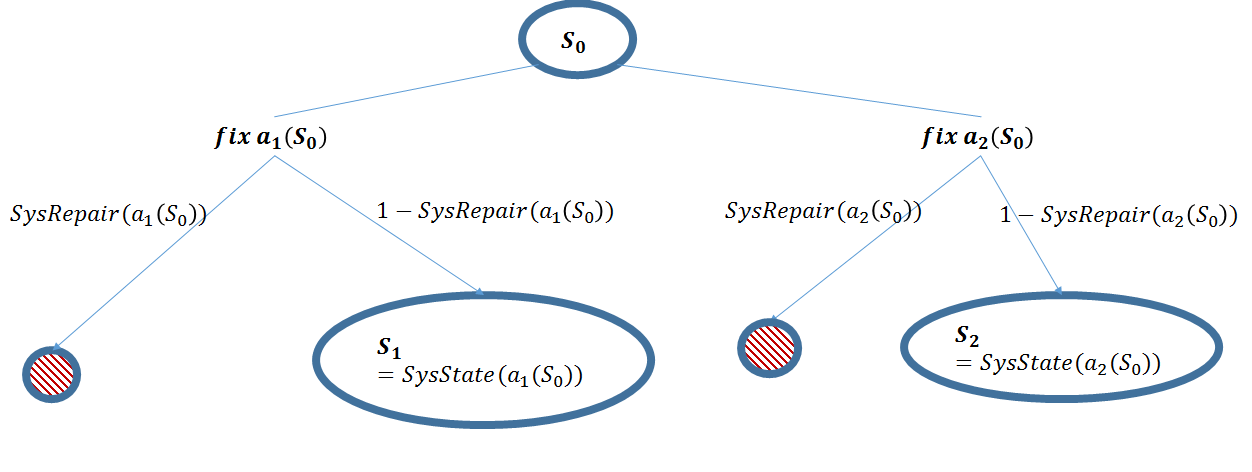
\includegraphics[width=0.8\columnwidth]{MDP.png}}
\caption{%TODO
}
\label{fig:MDP_example}
\end{figure}

 
 
Formalizing BRP as a SSP-MDP is useful because it allows using SSP-MDP solvers to compute the best (batch) repair action to perform. We elaborated on this next. 
 
%\subsection{Baseline MDP Solvers}
Baseline SSP-MDP solvers such as Value Iteration or Policy Iteration, require iterating over the entire state space in order to compute the optimal solution~\cite{russell2010artificialIntelligence}. 
Such approaches are not feasible for BRP, since the MDP state space for BRP is too large, as it represents all possible system states. That is, all subsets of components that may be repaired, and all possible observations that may be obtained after every repair action. 

Therefore, to solve our MDP problem we implemented an algorithm based on
the well-known Upper Confidence Bound for Tree algorithm (UCT)~\cite{kocsis2006bandit}, which has been applied successfully to solve large games and planning problems. Implementing UCT in practice involves several design choices. For completeness, we provide here a brief description of our UCT implementation and the design choices we made. 

\subsection{UCT for solving BRP}
UCT is designed to explore the MDP state space in a manner that balances \emph{exploration} and \emph{exploitation}, that is, it balances between exploring the outcome of actions not considered so far, and exploiting the knowledge gained so far about the state space. % and choose the best batch repair action. 
In every iteration of UCT, the algorithm explores a trajectory (a sequence of action and possible outcome) in the state space starting from the initial state and moving from one system state to the next by choosing a (batch) repair action. UCT uses the UCB (Upper Confidence Bounds) rule~(\cite{auer2002finite}) to choose an action in each tree node. 

\subsubsection{The UCB Rule}
The UCB rule requires maintaining for every explored state $s$ the number of times each state has been visited, denoted $NB_{s}$, as well as the number of times each action $a$ was taken in $s$, denoted $NB_{s,a}$. In addition, UCB requires a state-action vector $Q(s,a)$ that contains the average seen cost (reward) of taking action $a$ when in state $s$. With these values, UCB chooses the action that maximizes the following utility function:
\begin{equation}
U_s(a)= Q(s,a) + \alpha\cdot \sqrt{\frac{ln(NB_{s})}{NB_{s,a}}}
\label{eq:ucb}
\end{equation}
where $\alpha$ is a parameter. In our implementation, we set $\alpha$ to be the number of diagnoses in the initial state. \roni{It would be good to provide some intuition here for as to why we chose $\alpha$ like this.} We experimented with other possible values of $\alpha$ and found this to be the most effective in the experiments we performed.


Note that for actions that have not been chosen yet, $NB_{s,a} = 0$, which results in a division by zero in the UCB formula (Eq.~\ref{eq:ucb}). Thus, using the UCB rule results in always preferring to choose an action that has not been tried before over previously chosen actions. This is not a reasonable approach in our MDP, since the number of actions in a state is exponential in $|\notrepaired{}|$, and thus trying every action at least one will make this approach infeasible. This problem of initializing the $Q$ values is well-known in the literature, and approaches for solving it has been proposed~\cite{keller2012prost}. For our purposes, we defined the following BRP-specific initialization, which is used for actions that have not been chosen yet: 
\[ U_s(a)_0 = - \frac{cost_{FP}}{|a|} \]
Here too we explore several alternatives for 
such a \emph{default} utility function and found that the above worked well.

\subsection{Value Propagation}

In UCT, the values of the state-action vector $Q(s,a)$ for every state-action pair in the chosen trajectory needs to be updated. This is done in a bottom-up manner, i.e., starting from the last state-action pair in the chosen trajectory and propagating its value upwards. %This value propagation opens two design choices: how to set the value of in the bottom of the trajectory, and how to propagate it backwards. 

To control the running time of our UCT implementation, we limited the depth of the trajectory in each iteration, where this limit is a parameter denoted by $LH$. 
Thus, the last state in a chosen trajectory can be either a goal, i.e., when the system is fixed, or a state at depth $LH$. In case the final state is a goal state, which means that the system is fixed, the propagated value is initialized with 0, representing that no further repair costs will be incurred. If the final state is not a goal state, which means that  depth $LH$ has been reached, we defined the value of an action $a$ as 
\begin{equation}
    cost(a)=\sum_{c\in \notrepaired{}} F(c)\cdot(cost_{repair}+cost(c))
\end{equation}
%where $\overline{Repaired} \in s$ is the set of components that have not been repaired yet, as defined in Section \ref{sec:Repair_Likelihood}. 

Next, each state-action pair value $Q(s,a)$ is updated by accumulating the received values propagated from the lower levels of the trajectory, together with its immediate reward, $R(s,a) = -cost(Repair(a))$, and the resulted value is passed on to the level above. 

The number UCT iterations we run is a parameter. After completing the requested amount of iterations, the repair action eventually chosen is the one with the highest state-action value over all the state-actions pairs in the initial state.

\section{Experimental Results}
\label{sec:experimental-results}
%\meir{here add a short intro on the flow of this section.} 
In this section, we present an experimental evaluation of the proposed BRP algorithms, assessing their pros and cons, and demonstrating their benefit over baseline  approaches that do not allow batch repair actions. 
%We describe the experimental setup as well as the data and frameworks used to run the experiments. In addition, the results of the experiments will be presented, followed by observation and important trends derived from the results. 

%\begin{figure}{}%{4cm}
%\begin{center}
%  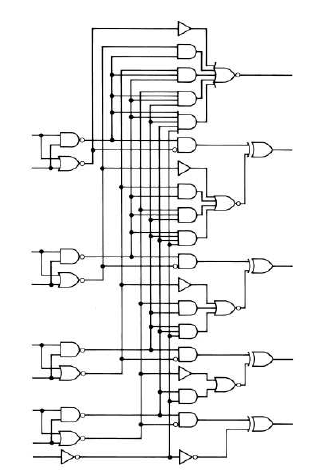
\includegraphics[width=0.5\columnwidth]{74283.png}
%  \caption{A logic diagram of ISCAS 74283 4-bit adder.}
%  \label{fig:74283}
%\end{center}
%\end{figure}


%Follow the introduction and experiments description, 
\subsection{Experimental Setup}

\noindent {\bf Domains.} We evaluated the proposed BRP algorithms on two different benchmarks. The first benchmark is the standard ISCAS 85~\cite{Brglez89} and 74XXX benchmarks~\cite{Hansen99}, which represent Boolean circuits. %\meir{the next fig and sentence is redundant } Figure \ref{fig:74283} presents a logic diagram of one of these systems called 74283, which is a 4-bit adder.
The system components (\COMPS) in this benchmark domain are the Boolean gates. The system description ($\SD$) includes the description of the components' behaviors. For instance, the healthy behavior of an $\textit{OR}$ gate is the logical OR operation, while abnormal behaviors can be stuck at 1, stuck at 0, or flip (i.e., outputting the opposite of the normal output). An observation ($\OBS$) in this domain is the inputs and outputs values of the system. A diagnosis states which gates are healthy and which are in a faulty mode. Our BRP algorithms output a set of gates to fix. 

\begin{table}\centering
{\small
\begin{tabular}{|l|r|r|r|r|}
\hline
 {\bf Name} & {\bf $|${\tiny \COMPS}$|$} & {\bf in} & {\bf out} & {\bf \#observations} \\
\hline
    74182  & 19    & 9    & 5    & 25 \\
    74283  & 36    & 9    & 5    & 22 \\
\hline
    c432   & 160   & 36   & 7    & 23\\
    c880   & 383   & 60   & 26   &  30\\
\hline
\end{tabular}
\caption{Details on the Boolean circuits benchmark used in our experiments. THe systems are from the {\small 74XXX} and {\small ISCAS-85} systems, and observations from DXC'09~\cite{feldman2010approximate}.}
\label{tab:systems}
}
\end{table}%


Details of the standard Boolean circuits we used in our experiments are presented in Table \ref{tab:systems}. The systems {\small 74XXX}~(\cite{Hansen99}) are described in the first two rows, and additional two systems of {\small ISCAS-85} (\cite{Brglez89}) are described in the following two rows. Observations were selected randomly from Feldman et al.'s~(\shortcite{feldman2010approximate}) known benchmark of observations.

%\meir{i added more details on this section}
%Physiotherapy
The second benchmark domain we used is from the medical physiotherapy field. The model was elicited on the upper human body which is innervated by the nerve roots $\operatorname{C-3}$ to $\operatorname{T-1}$, or from head to the upper part of the torso. 
\roni{I dont understand this sentence. (1) what doe sit mean that a ``model was elicited on ...''? I don't see how ``elicited'' fits here. 
(2) How can C-3 to T-1 be a range? I understand a range 1-3 and a range A-C but what's C-3 to T-1?}
The information was acquired through interviews with senior physiotherapists and data gathering from physiotherapy graduate students. $COMPS$ in this model are the \textit{Nerve roots}, \textit{nerves}, \textit{muscles} and \textit{dermatomes}. $SD$ describes the relations between the different entities are described in Figure~\ref{fig:entities}. $OBS$ are the patient's weakened motions or defected sensations. The data used in our experiments was obtained from simulations of medical physiotherapy cases of human patients. In total, we have experimented on more than 500 observations. 

\begin{figure}[h]
 \centering
 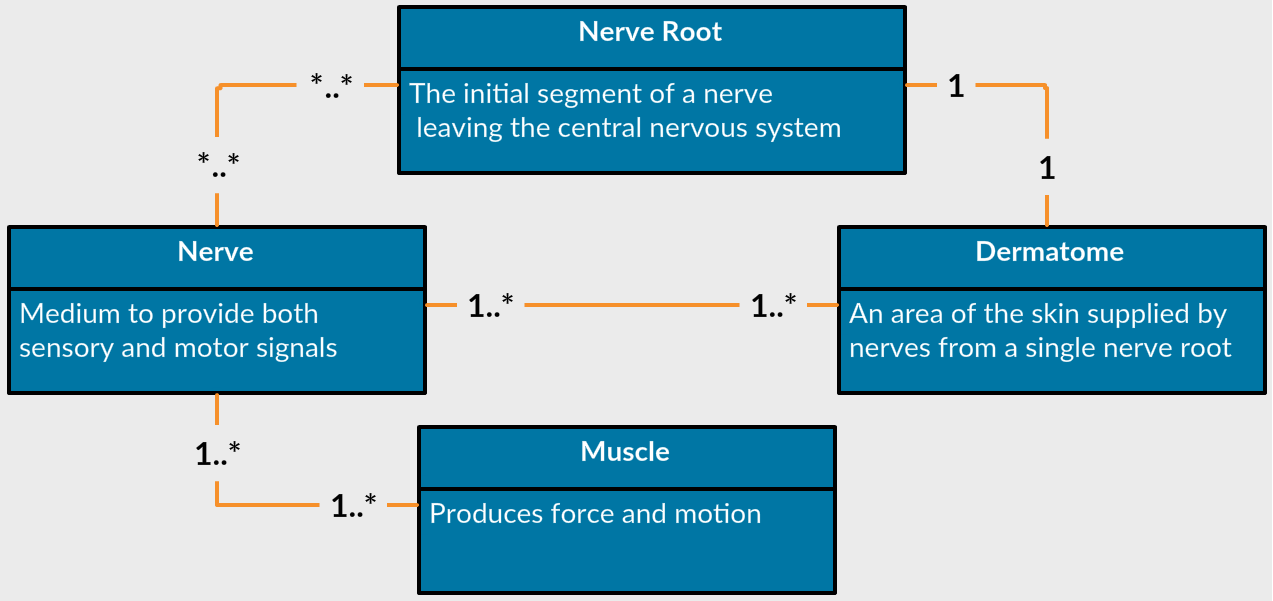
\includegraphics[width=10cm]{Entities.PNG}
 \caption{Anatomical entities represented in the diagnosis models.}
 \normalsize
        \label{fig:entities}
\end{figure}

%parameters - prior probability and costs
\noindent {\bf Parameters.} In both domains, we set the prior probability of each component to be faulty to 0.01 and chose a single diagnosis for each observation to serve as the real injected faults. This is needed to decide when the system is fixed. Note that this ``true'' diagnosis was chosen with probability proportional to its likelihood of being correct, computed according to the priors mentioned above under the standard assumption of fault independence. The component repair cost was set to 5, and we experimented with repair overhead ($cost_{repair}$) costs of 5, 10, 15, 20, and 25.

Some of the evaluated algorithms require predetermined parameters. In particular, some of the search-based algorithms have a \emph{bound} parameter that specifies the maximal number of diagnoses to consider repairing (the union of the components). Our UCT implementation also requires parameters: the lookahead depth ($LH$) 
and the number of iterations. 
After some parameter tuning, we used a bound of up to 3 for the search algorithms, and $LH=5$ and 10,000 iterations for our UCT. 


%diagnoses generation and cardinality:
\noindent {\bf Diagnoses generation and measure.} For every observation, we computed a set of corresponding diagnoses. In the physiotherapy domain we considered all the subset minimal diagnoses.  
In the Boolean circuits domain we further limited the set of diagnoses to include only the minimal cardinality diagnoses, since the set of all subset minimal diagnoses was too large. 

To compare between the different BRP algorithms, we measured their total cost as follows. 
For every observation we run a BRP algorithm which chooses a batch repair action. Then we performed this repair action. If the system is not fixed yet, then we run again the BRP algorithm to choose the next batch repair action. This process continues until the system is fixed. The cost of the BRP algorithm was determined by the overall costs incurred by these repair actions. We limited the runtime of all algorithms to 5 minutes. 
An algorithm that reached this timeout was forced to return the best repair action it found so far. 

%\meir{I would not explain here about this experiment, but before you present the results for this benchmark, you can introduce the reason we chose a subset of the observations.} -done
%Although we had a large set of observations to run our experiments on, we decided to sample a portion of the bunch for our experimental phase. The reason for that is mainly because of the trade-off between run time and results quality. By analyzing the data we noticed that the full set of the observation can be divided into several equivalent classes. In each class, there is a relatively low variance to the resulted cost obtained from using a repair algorithm on the observations. On the other hand, running the algorithms on all of the observations take a significant amount of time and resources. Therefore, by considering this trade-off we decided that it is more beneficial to use a portion of the observations set. 
%In addition, we ran another set of experiments on the chosen portion of the obtained data, which included only the observations in which the matching set of diagnoses size did not exceed 30 diagnoses. That is because the computation complexity depends mostly on the size of the given set of diagnoses, and by adding the mentioned restriction criterion for the experimented cases we could reduce the number of times the algorithms reaches the timeout limitation, and by that increases the percentage of cases in which the optimal solution is returned. 

\noindent {\bf Evaluated Algorithms.} 
%\meir{here you should set the abbreviation of the algorithms you use later. So when the reader sees, for instance, in a graph the abbreviation "KHighestProb\_1", he could look here to see what you mean. Therefore, you should add here some more details. This is actually a summary for the reader to remind him what is each algorithm or objective function. Only one sentence for each - but it helps.}


We have evaluated the next BRP algorithms:
\begin{enumerate}
\item Search-based algorithms: 
\begin{enumerate}
\item Uninformed search ({\bf Union-K}). 
\item Heuristic search algorithm:
\begin{enumerate} 
\item Hill Climbing ({\bf HC}).
\item Optimal search ({\bf A*-Union}).
\end{enumerate}
Each one of heuristic search algorithms was experimented using three different objective functions ("Optimistic", "Pessimistic" and "Pessimistic FFP Enhanced"). 
\end{enumerate}
\item MDP based algorithm ({\bf MDP}).
\item Baseline algorithms: 
\begin{enumerate} 
\item Best Diagnosis ({\bf BD}) which chooses to repair all components in the most likely diagnosis in a batch repair action. 
\item K-Highest Probability ({\bf K-HP}), which chooses to repair the K components with the highest probability to be faulty according to the Health State.
\end{enumerate}
\end{enumerate}

The main hypothesis of this line of work is that performing batch repair actions can save repair costs, comparing to a repair action of a single component. Thus, we compare our BRP algorithms to {\bf 1-HP}, in which the component that is most likely to be faulty is repaired. A similar approach was used by previous work on test planning~(\cite{zamir2014using}). 

\subsection{Results}
%\meir{it is not a good way to start this section. At the end of the section "The Benefit of Batch Repair" you can mention that the rest of the results are presented in the appendix. Also the next comment is not necessary here, but when you present the first graph you should say that we used the "Pessimistic FFP Enhanced" wasted cost utility function, and add that in all this section we presents the results with this function , unless mentioned otherwise. Instead of these comments you should describe the flow of this section. What results we are going to see. something like: "In this section we will present the results of the BRP algorithms. In Section \ref{sec:benefit-BR} we will demonstrate the benefit of the batch repair algorithms over a single repair...etc."} -done
%Tables presenting the results can be found in the appendix.
%Note that the results of the search-based BRP algorithms that are presented in tables and charts refers to results achieved using the "Pessimistic FFP Enhanced" wasted cost utility function, unless mentioned otherwise. 
In this section we will present the results of the BRP algorithms. In Section \ref{sec:benefit-BR} we will demonstrate the benefit of the batch repair algorithms over a single repair. Then we will compare between our proposed batch repair algorithms. We will attempt to shed a light on the superior features of the algorithms which obtained the best results. We will try to detect the optimal conditions for choosing the best algorithm for a given situation. Finally, we will discuss our conclusions arising from the results. 

%1-single vs batch results:
\subsubsection{The Benefit of Batch Repair}\label{sec:benefit-BR}


Figures ~\ref{fig:P-batch-base-single} and ~\ref{fig:I-batch-base-single} plot the average repair cost (y-axis) for each repair algorithms (x-axis) for the ISCAS and the Physiotherapy domains, correspondingly. 
%\meir{you should mention what parameters are fixed in the figures and what are varied.} -done. %for all the figures? 
We run the A*-Union with the Pessimistic FFP Enhanced objective function. %, with the bound set to 3, which is also the bound of the results represented by the MDP column. 
Figure ~\ref{fig:P-batch-base-single} shows the results with different values of the overhead cost parameter, and in Figure ~\ref{fig:I-batch-base-single} it was set to 25. 


%Additional charts of the results are presented in order to demonstrate this trends visually;

\begin{figure}[h]{}
\centering
\frame{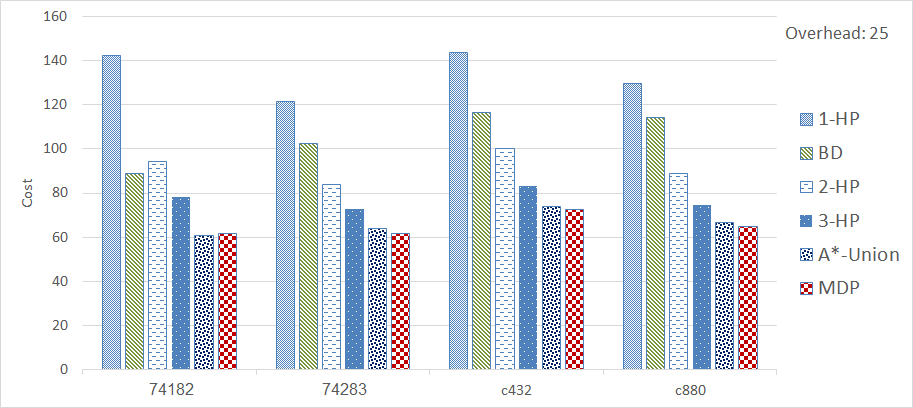
\includegraphics[width=0.8\columnwidth]{Charts/I7_color_1.png}}
  \caption{ISCAS: Average repair costs when the overhead cost is set to 25.
}
  \label{fig:I-batch-base-single}
\end{figure}

\begin{figure}{}
\centering
\frame{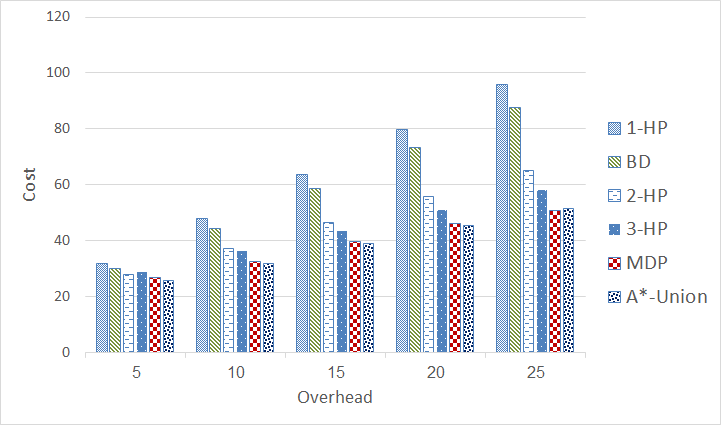
\includegraphics[width=0.8\columnwidth]{Charts/P7_color_1.png}}
  \caption{Physiotherapy: Average repair costs for different overhead costs.
}
\label{fig:P-batch-base-single}
\end{figure}

These results support our main claim that reasoning about the possibility of batch repair is beneficial. The BRP algorithms cost-effective than the baseline algorithms. 
As shown in figure~\ref{fig:P-batch-base-single}, increasing the repair overhead cost causes all algorithms to require an increasing cost to fix the system. Nevertheless, the advantage of batch repair algorithms over 1-HP increases as the repair overhead cost increases, demonstrating that the cost-effective of batch repair is greater when the overhead costs are higher. 

For example, in the experimental results in the physiotherapy domain, running algorithm A*-Union with an overhead cost of 20 required a cost of 43 on average, while 1-HP with the same setting required 79.8 which is almost twice as much.
Another good example from the ISCAS domain (system 74182), while all the unbounded batch repair algorithms required on average a total cost of 59.1, when the overhead cost was set to 25, the 1-HP with the same overhead required 142.3.

%\begin{figure}{}
%\frame{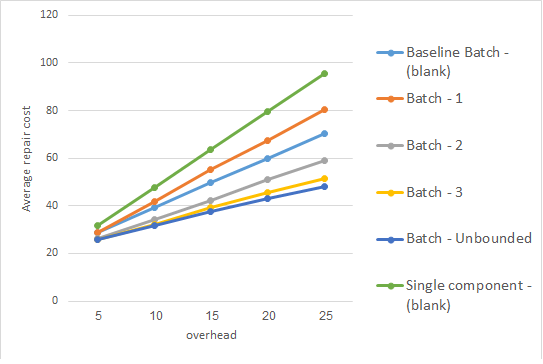
\includegraphics[width=0.8\columnwidth]{Charts/P_batch_base_single_graph.png}}
%  \caption{Average repair costs of physiotherapy cases experimental results using batch (bounded and unbounded), baseline and single component repair algorithms, with different overheads.}
 % \label{fig:P-all-graph}
%\end{figure}



%\subsection{Comparison of Batch Repair Algorithms}
%2-batch algos vs base
%Next, we compared the performance of our search-based BRP algorithms and our UCT-based BRP algorithm
%against the baseline algorithms, K-HP and BD-Batch.
%In Figure~\ref{fig:P-batch-base}, Figure~\ref{fig:I-batch-base-single} and ~\ref{fig:P-BD-UK} plots the overhead cost on the X-axis and the average repair cost on the Y-axis. We can see in those charts the large gap between the A*-Powerset algorithm to the rest, which grows more and more as the overhead grows. 

%The results in Figure~\ref{fig:P-BD-UK} show the benefit our our WC utility function compared to the simpler BD-Batch algorithm. The results show a clear advantage of our Union-based search algorithms even when limiting it to bound 1. 
%For example, in the experimental results of the physiotherapy domain, Union-based search algorithm and overhead 20 required cost of 67.6 on average, while BD-Batch on the same setting required 73.3.

%These results highlight the benefit of our proposed utility functions for evaluating a repair action candidate. That is because the difference between BD-Batch and Union-based search with bound 1 is that BD chooses the diagnosis to repair according to its probability to be correct and not according to our WC utility function. 


%\begin{figure}{}
%\frame{\includegraphics[width=0.8\columnwidth]{Charts/P_BDvsUK.png}}
%  \caption{Average repair costs of physiotherapy cases experimental results Union-1 vs BD with different overheads.}
%  \label{fig:P-BD-UK}
%\end{figure}

\begin{figure}{}
\frame{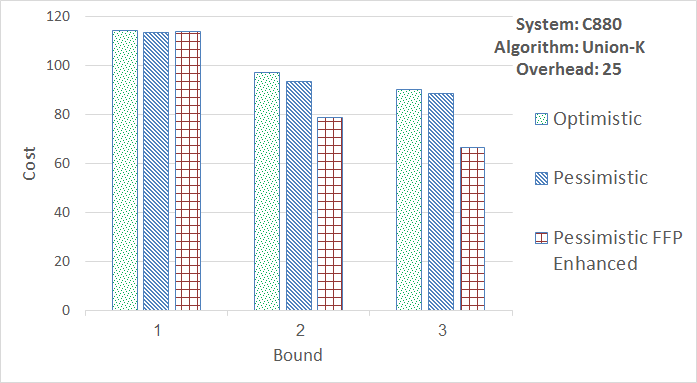
\includegraphics[width=0.8\columnwidth]{Charts/I11_color.png}}
  \caption{%\meir{add caption to the y axis} -done
  ISCAS system c880: Average repair costs of Union-K algorithm with different bounds and different wasted cost utility functions.
  }
  \label{fig:I-obj}
\end{figure}

\begin{figure}{}
\frame{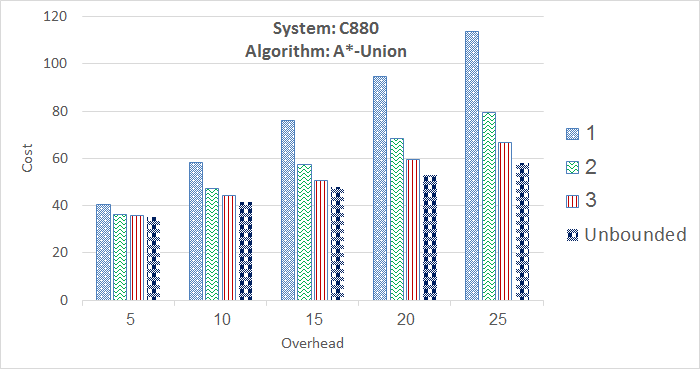
\includegraphics[width=0.8\columnwidth]{Charts/I12_color.png}}
  \caption{%\meir{add caption to the y-axis} - done
  ISCAS system c880: Average repair costs of Union-K algorithm with different bounds and different overhead costs.}
  \label{fig:I-bounds}
\end{figure}

\begin{figure}{}
\frame{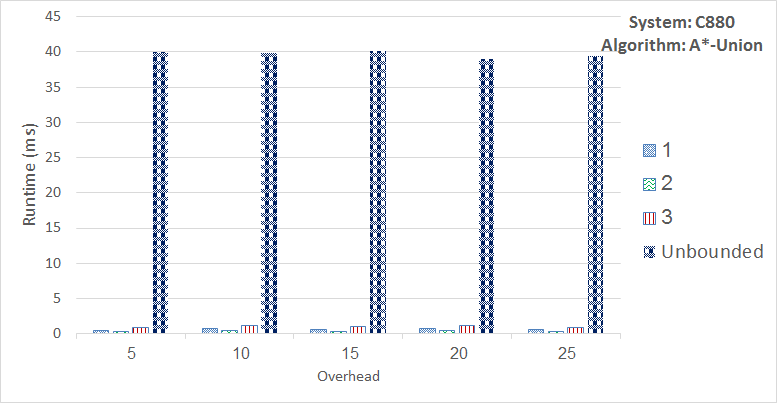
\includegraphics[width=0.8\columnwidth]{Charts/I12_runtime.png}}
  \caption{ISCAS system c880: Average runtime of Union-K algorithm with different bounds and different overhead costs.}
  \label{fig:I-bounds_runtime}
\end{figure}

%\subsection{Comparison of WC Utility Functions}
\subsubsection{BRP Search-Based Algorithms}
In this section we present results that show the impact of different factors on the search-based algorithms.

Figure~\ref{fig:I-obj} presents the %significant differences between the 
impact of the way we compute the wasted cost utility functions. The results are presented for ISCAS system C880, where the overhead cost is fixed to 25. The x-axis represents the different bounds of the Union-K algorithm, and the y-axis represents the average repair cost. It seems that the lowest average repair cost is achieved when using the Pessimistic FFP Enhanced wasted cost utility function. We believe that the main reason is that it takes into consideration the future mistakes: by analyzing the possible impact on the future the estimated utility can potentially be closer to the actual future occurrences.

Note that when the bound is 1 there is no significant difference between the wasted cost utility functions. \meir{i dont understand the next sentence} The reason is that there is a small variance in effected repair costs and future actions. The chosen repair action in each round could be composed of only one diagnosis, and by that any choice would reduce the search space by a similar scale. \meir{same for the next sentence} Moreover, we should not disregard the similarities between the wasted cost utility functions, as all of them consider the False Positive costs. In any case, limiting the possible actions, reduces the variance of the different potential outcomes.
%For example in figure~\ref{fig:P-obj-15}, the results of the search based algorithms with bound of 3 when using the pessimistic enhanced utility function has yielded an average repair costs of a little less then 40, while the use of the optimistic utility function by the same algorithms got the average repair cost to exceed 50.

%search bounds
Figure~\ref{fig:I-bounds} plots the average repair cost (y-axis) as a function of the different bounds of A*-Union algorithm for various of overhead costs (x-axis). Increasing the bound of the search-based BRP algorithm minimizes the total repair costs. 
This trend is expected, since increasing the bound causes a wider set of possible repair actions, and as a result a higher chance of covering more faulty components in one repair action.
Even though the minimal repair costs can be achieved by unbounding the search space, the runtime of the search algorithm would skyrocket. One should consider the trade-off between the costs and runtime of the unbounded vs bounded search. 
Figure~\ref{fig:I-bounds_runtime} plots the bound of A*-Union algorithm on the x-axis and the average runtime on y-axis, where the runtime penalty of unbounded search is vividly depicted.
%Nevertheless, considering the runtime of the search algorithms with unbounded search space, 

\subsubsection{Comparison of Search-Based and MDP-Based Approaches}

%\begin{figure}{}\frame{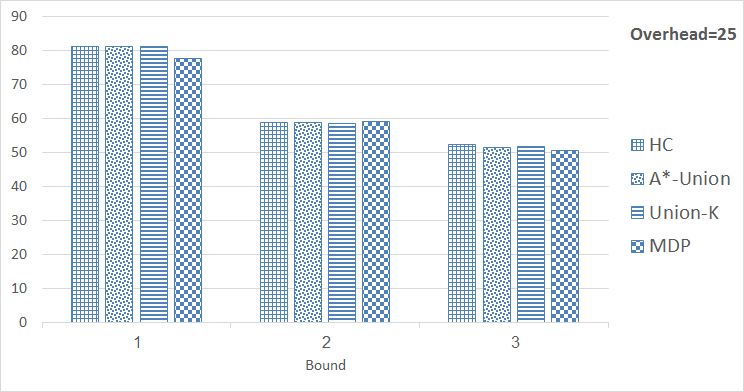
\includegraphics[width=0.8\columnwidth]{Charts/P13.png}}\caption{%TODO}\label{fig:P-search-MDP}\end{figure}

\begin{figure}{}
\frame{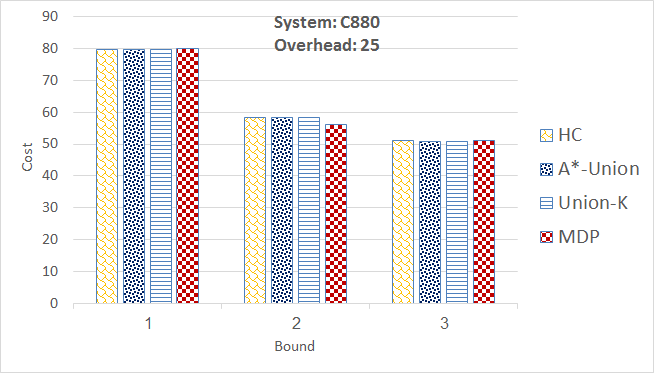
\includegraphics[width=0.8\columnwidth]{Charts/I13_notimeout.png}}
\caption{%\meir{add caption to the y-axis} - done
ISCAS system c880: Average repair costs of search-based and MDP algorithms with different bounds where the overhead cost is 25.
}
\label{fig:I-search-MDP}
\end{figure}

%\begin{figure}{}\frame{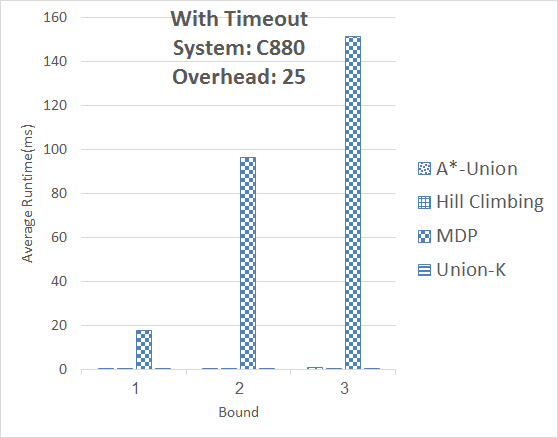
\includegraphics[width=0.8\columnwidth]{Charts/I14TO.png}} \caption{%TODO}\label{fig:I-runtime}\end{figure}

\begin{figure}{}
\frame{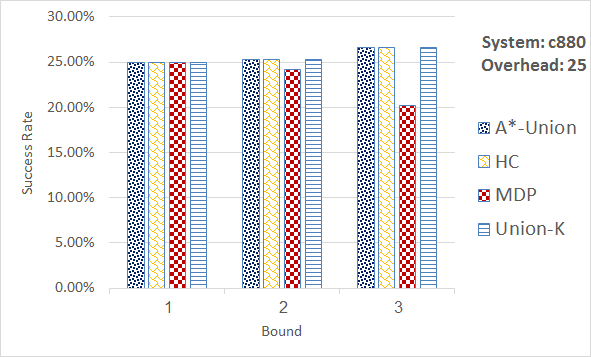
\includegraphics[width=0.8\columnwidth]{Charts/I15_suc_rate.png}}
  \caption{%\meir{present the success rate rather than the number of successes} -done
ISCAS system c880: Success Rate of search-based and MDP algorithms with different bounds where the overhead cost is 25.
}
  \label{fig:I-success-rate}
\end{figure}


%There are few observations to discuss after analyzing the results of the search-based and MDP-based algorithms.
Figure~\ref{fig:I-search-MDP} presents a comparison between the search-based and the MDP-based algorithms. The x-axis represents three bounds and the average repair cost is indicated by the y-axis.
%plots the bound of the algorithms on the x-axis and the average repair cost on y-axis.
%As depicted int figure ~\ref{fig:I-search-MDP}, in the repair costs comparison between the algorithms, 
%The results appear to be very close.%\meir{does Figure~\ref{fig:I-search-MDP} present the cost for all the 90 cases? or only for the cases where all algorithms finished to run in the time limit of 5 minutes? we should present here the second option. I hope that after you update it we will see an advantage to the MDP, and then we can show the tradeoff between success rate and cost, otherwise we should rethink about the advantage of MDP. hilla: updated to the second option} 
It seems that there is no significant difference between the methods. It is expected that the average repair cost will be the same for the three search-based algorithms since they all bounded by the same depth. However, the MDP ...\meir{...why is not better?}. 

We examine also the success rate in a 5 minutes limit of the algorithms in Figure~\ref{fig:I-success-rate}. The algorithm's bound is indicated in the x-axis and the number of successes in the y-axis. MDP-based algorithms grows exponentially, and thus we can see here that the success rate of the MDP-based BRP algorithm decreases.  
%Note that the MDP based algorithm does hold an advantage regarding using an objective function to estimate the utility of a repair action, since the other algorithms need to be received with a predefined one, while make this estimation on its own.
%We would not suggest that there is a clear winner among the batch repair algorithms, as it probably depends on the domain, the needs and the environmental restrictions. 


\subsection{Experimental Results Summery}

To summarize, we observed the following trends:
\begin{itemize}
\item All batch repair algorithms yield significantly better results than the single repair algorithm, and the gap grows as the overhead cost gets larger.  
\item Our proposed BRP algorithms triumph the baseline batch repair algorithms.
\item Bounding the search-based algorithm reduces the runtime performances, in the expenses of increasing the repair costs. 
\item The best results of the search-based algorithm are achieved by using Pessimistic FFP enhanced utility function, which is used to estimate the false negative cost.
%The best results of the search-based algorithm are achieved by using the wasted cost utility function, where the Pessimistic FFP enhanced is used to estimate the false negative cost.\meir{why not saying: "The best results of the search-based algorithm are achieved by using Pessimistic FFP enhanced utility function, which is used to estimate the false negative cost."}%, in order to estimate the merit of a repair action.
%\item The average repair cost results of the MDP algorithm are the lowest, though its success rate is smaller than the rest algorithms.%\meir{we should verify this result}
\end{itemize}

\section{Related Work}
\label{sec:relatedWork}	
BRP is a troubleshooting problem, where the goal is to perform repair actions in order to fix an abnormally behaving system. Algorithms for automated troubleshooting were proposed in previous works. Most previous work assumed that components are repaired one at a time ~(\cite{heckerman1995decision,friedrich1992choosing,Nyberg12,Torta14}). This approach can be wasteful for BRP. For example, if a diagnosis engine infers that multiple faulty components need to be repaired to fix the system, then it would be wasteful to repair these components one at a time since each repair action incurring its repair overhead. Instead, an efficient BRP algorithm would repair all the faulty components in a single repair action. 


In troubleshooting, there are two main areas. The first is the Diagnosis, which focuses on the part in the troubleshooting process that searches the possibilities of explanations to what could have cause the system's malfunction. The second is the Planner, which focuses on planning the actions that follows the diagnosis phase, such as reducing the number of diagnoses, deciding what will be the next repair action etc. This chapter will present related work from various areas and lines of works in troubleshooting. The first part of this chapter will discuss related troubleshooting processes and algorithms. The second part will present diagnosis approaches, while focusing on the field of Model-Based Diagnosis. Finally, the last part will present related work from the planning filed and will elaborate about different planner algorithms and approaches. 

\subsection{Diagnosis Approaches}
There are diverse diagnosis approaches such as data-driven, case-based reasoning, and model-based diagnosis.


Data-driven approaches are model-free statistical methods, which attempt to learn relations between the symptoms and the faults ~(\cite{murray2005machine}). These methods face the challenge of a dependency of the existence of quality information that can be extracted from the data. One disadvantage of most works in this approach is that they learn only a single fault rather than multiple faults. In addition, inductive learning methods do not guarantee sound diagnoses nor completeness.


Another approach is case-based reasoning. Experts often find it easier to relate stories about past cases rather than to formulate rules. Case-based reasoning methods keep a repository of cases and their appropriate diagnosis. When a new case appears the case-based reasoning system tries to find the most similar case from the repository in order to adapt the relevant diagnosis ~(\cite{aamodt1994case}). The main assumption is that similar problems have similar solutions. Similar to data-driven approaches, this approach also does not guarantee sound diagnoses nor completeness. Thus, one could not be certain that the resulting diagnosis is indeed the faulty component.
In this work we focus on model-based diagnosis approach (MBD)~(\cite{reiter1987theory}).


In MBD we must have a precise model of the system. MBD relies on a model of the diagnosed system to compute the expected behavior of the system. When the expected and observed behavior differs, the model is used to infer possible failing components ~(\cite{reiter1987theory}).
The Model Based Diagnosis problem with weak fault model has been widely researched and a wide range of papers propose different algorithms to solve it ~(\cite{reiter1987theory,de1987diagnosing,williams2007conflict,feldman2010approximate,siddiqi2007hierarchical}).


Many of the existing diagnosis techniques propose to apply a combination of deterministic reasoning and search algorithms. One classic approach involves a two stage process. First, it identifies conflict sets, each of which includes at least one fault. Then, it applies a hitting set algorithm to compute sets of multiple faults that explain the observation~(\cite{de1987diagnosing,williams2007conflict}). These methods guarantee sound diagnoses, and some of them are even complete. However, they tend to fail for large systems due to infeasible runtime or space requirements.
Compilation-based methods have also been proposed in the MBD context. Torasso and Torta apply binary decision diagrams (BDD) to compile the model ~(\cite{torasso2006model}). Darwiche ~(\cite{darwiche2001decomposable}) compiles a system description into Decomposable Negation Normal Form (DNNF) where a minimal cardinality diagnosis can be found in time that is polynomial in the size of the DNNF. This compilation approach is attractive because inference of diagnoses can typically be done in time that is linear in the size of the compiled representation; however, there is no guarantee that the size of the compiled representation will not be exponential in the number of system components. Other work proposes to compile MBD to the SAT problem ~(\cite{metodi2012compiling}), and then use state-of-the-art SAT or MAX-SAT solvers to find the possible diagnoses. 
In this work, in order to find the possible faulty components, we will use the MBD approach in the implementation of the diagnosis engine.  

\subsection{Troubleshooting Planner}
There are two lines of work that study planning algorithms in the context of troubleshooting. The first is probing and testing, which are the two known methods for reducing the number of diagnoses after they are found. In the second line of work, there is a use of planning in order to decide which possible repair actions can be taken next. BRP algorithms are a part of the second line of work. 

\subsubsection{Probing and Testing}
Some methods try to deal with reducing the number of diagnoses after they are found. There are two known methods to discriminate diagnoses, either by testing or probing ~(\cite{de1987diagnosing}). In the testing method the diagnosis process is run through additional input vectors. Under the assumption that faulty components in the system remain permanently faulty along different input vectors, diagnoses that are inconsistent with multiple observations can be pruned. The probing task is similar, but instead of running the diagnosis on a new input vector, the probes are requests on the observation of the output of internal components. Probes can prune diagnoses that are not consistent with the new internal observation. Both methods can be run iteratively until focusing on a single diagnosis.
Zamir, Stren and Kalech~(\cite{zamir2014using}) proposed a combination of AI techniques to improve software testing. In this domain, the diagnoses represents a set of possible explanations to a failed test, and a planning algorithm is used to suggest further tests to identify the correct diagnosis. They describe an iterative course of action which prunes incorrect diagnoses in each iteration while using an MBD algorithm. This iterative process, which they call Test, Diagnose and Plan (TDP), continues until the correct diagnosis is returned. Several test planning algorithms are proposed to minimize the number of TDP iteration, and consequently the number of tests required until the correct diagnosis is found. 


Torta et al.~(\cite{Torta14}) proposed using model abstractions for troubleshooting and point out the role of abstractions in an iterative abduction process. Similar to Model-Based Diagnosis and troubleshooting, at each iteration of the abduction process the proposed algorithm in their work chooses to perform further observations or actions taking into account their costs and the likelihood candidate hypotheses.

The planning role in the troubleshooting processes described above is to reduce the number of diagnoses by finding and pruning incorrect ones. In the BRP the goal of the planning algorithms in each iteration of the troubleshooting process is to find the right component to repair so the system will be fixed as soon as possible, meaning eventually fixing all the correct diagnosis' components. 


\subsubsection{DTT Planner}

%\roni{you already mention this planner above. The structure of the related work section needs work. Try to make it more coherent. Start with the diagnosis stuff, then the troubleshooting.} hilla-done

Heckerman et al.~(\cite{heckerman1995decision}) proposed the decision-theoretic troubleshooting (DTT) algorithm that uses a decision theoretic approach for deciding which components to observe in order to identify the faulty component. Later work also applied a decision theoretic approach that integrated planning and diagnosis to a real world troubleshooting application~(\cite{Nyberg12,warnquist2009planning}). 
The diagnostic procedure developed by Heckerman et al.~(\cite{heckerman1995decision}) not only seeks to identify the most likely causes of a malfunction, but also generates a plan of action for repair. This plan consists of repairing or replacing individual components of a composite device or system, as well as making observations or tests. This is essentially the troubleshooting process. An optimal troubleshooting plan, as described in their work, is a sequence of observations and repairs that minimizes expected costs. The classic way to compute the expected cost of a plan is to use a decision tree. The decision tree contains: decision nodes that represents of whether or not to observe variable o, chance nodes of each o which represents an observation that provides some evidence about the status of the components and its branches represent the possible outcomes of the variable, and decision nodes that represents the decision of whether or not to fix the component c. The values at the end of the tree are cumulative costs of observation and repair along the path from the root. The expected cost of a troubleshooting plan is computed by rolling back a decision tree from right to left – a particular form of dynamic programming. After all the computations has been done, there will be a chosen action for each decision node and ultimately will represent the optimal plan. 
The possible decisions that can be made, after assembling the optimal plan derived from a decision tree, can only integrate repair action that contains only one component. In BRP, the idea is to consider repairing more than one component in each repair action. The decision tree grows exponentially as the problem grows. This applies for cases in which the upper bound of the amount of possible repair actions is the number of components. Imagine how the tree will look like in cases, such as BRP, where the amount of possible repair actions that is exponential with the number of components. In other words, using decision tree to solve BRP in most cases is not feasible. 


Pernest{\aa}l et al. ~(\cite{Nyberg12}) work was motivated by the task of repairing an automotive vehicle at lowest possible expected cost, and proposed a decision theoretic troubleshooting system that is developed to handle external interventions. Warnquist et al.~(\cite{warnquist2009planning}) studied the problem of incremental fault diagnosis and repair of mechatronic systems where the task is to choose actions such that the expected cost of repair is minimal. This is done by interleaving acting with the generation of partial conditional plans used to decide the next action.

\subsubsection{Breakdown Costs}
Some of the previous works in this line of work considered also the costs. Friedrich and Nedjl~(\cite{friedrich1992choosing}) discussed the relation between diagnoses and repair, in an effort to minimize the breakdown costs. Breakdown costs roughly correspond to a penalty incurred for every faulty output in the system, for every time step until the system is fixed. In BRP, the goal is to minimize costs until the system if fixed, and there is no partial credit for repairing only some of the system outputs.

%\section{}

None of these works considered the possibility of repairing a set of components together, allowing only repair actions that repair a single component at a time.
%\roni{Remove the next two paragraphs. Your thesis summarizes all our work. You don't need to discuss how it relates to some preliminary workshop paper that we did}
%Recent work of Stern and Kalech~\cite{stern2015repair} proposed two high-level approaches to solve BRP: as a planning under uncertainty problem, or as a combinatorial optimization problem. When modeling BRP as a planning under uncertainty problem the task is to find a repair policy, mapping a state of the system to the repair action that minimizes the expected total repair costs. This approach, while attractive theoretically, quickly becomes not feasible in non-trivial scenarios.

This work do not consider applying further diagnostic actions such as probing and testing, which are considered by previous troubleshooting algorithms. Thus, this work could be integrated in previous troubleshooting frameworks in order to consider both batch repair actions and diagnostic actions. This is left to future work.

\section{Conclusion and Future Work}

We addressed the problem of troubleshooting with the possibility of performing a batch repair action --- a repair action in which more than a single component is repaired. Batch repair makes sense only if repairing a set of components in a single repair action is cheaper than repairing each of them separately. We proposed several algorithms for selecting which batch of components to repair. Experimental results clearly show the benefit of batch repair over single repair actions, and the benefit of the algorithms we suggested for choosing these set of components to repair. Furthermore, the results has demonstrated that the importance of batch repair is greater when overhead costs are higher.  

The computation of the proposed utility functions embodied several assumptions. First, components are assumed to fail independently (this is used in Equation~\ref{eq:likelihoods}). Second, we assume that a batch repair action always succeeds, i.e., all repaired components are healthy after it. Third, we assume that overhead cost does not depend on the components being repaired. 
%In future work we will investigate how relaxing these assumptions.


%objective functions:
In addition, comparing the experimental results of the search-based algorithms to the baseline algorithms, amplifies the importance of using our proposed utility functions in order to evaluate a repair action candidate. Furthermore, using the wasted cost utility function, which uses the Pessimistic FFP enhanced to estimate the false negative cost, resulted with the lowest average repair costs, which makes it the best utility function among the proposed functions so far. Note that the presented trend suggests that the more pessimistic is the estimation, the better. Future work can include testing the "pessimistic bound" in which making the estimation more pessimistic will be resulted with higher repair costs. 



%BRP algorithms:
We proposed search-based algorithms that attempt to find the best repair action, and tested their performances with different bounds, as well as without bounding the search space. The results showed that by increasing the bound, we can minimize the total repair costs. 
Furthermore, the search algorithms with unbounded search space had better results, in terms of the resulted repair cost, than those with a bound. Although not bounding the search space can achieve better results cost wise, we can reduce the runtime of the algorithm significantly with bounding the search. In the discussion of this trade-off between cost and runtime, the benefit of bounding the search space became very clear, due to the small differences in the resulted costs, and large differences in the total runtime of the algorithms. 

Additionally, We proposed an alternative approach to address the batch repair problem as a planning under uncertainty problem, which we modeled as a Markov Decision Process (MDP) and solved it appropriately. A clear advantage to the MDP algorithm over the search-based algorithms is that the search-based algorithms need a predefined objective function to estimate the utility of a repair action, while the MDP makes this estimation on its own.
Nevertheless, we would not suggest that there is a clear winner among the batch repair algorithms, as it probably depends on the domain, the needs and the environmental restrictions.

%after thesis review-not enough:
Future work could be evaluating the proposed approaches experimentally on a realistic domain, and maybe sharpen the differences, strength and weaknesses of the various BRP algorithms. Additionally, there is a potential for composing  new utility functions, using various approaches for evaluating a repair action. 


%\subsubsection*{Acknowledgments}


%\bibliographystyle{theapa}
%\noindent {\bf References.}
\section*{Bibliography}
\bibliography{batch-repair}

\section*{Appendix}

%results tables:
\begin{table}[]
\centering
\caption{Experiments results on Physiotherapy cases: Average repair costs until the system is fixed}
\label{tab:physioRes}
\begin{tabular}{|l|l|l|l|l|l|l|}
\hline
\multicolumn{2}{|l|}{}                                                          & \multicolumn{5}{c|}{\textbf{Overhead Cost}}                        \\ \hline
\textbf{}                                           & \textbf{Algorithm} & \textbf{5} & \textbf{10} & \textbf{15} & \textbf{20} & \textbf{25} \\ \hline
Single Component                                           & 1-HP     & 31.9       & 47.9        & 63.8        & 79.8        & 95.7        \\ \hline
Baseline                                                   & BD & 29.9       & 44.4        & 58.8        & 73.3        & 87.8        \\ \hline
Baseline                                                   & 2-HP     & 27.8       & 37.2        & 46.5        & 55.9        & 65.2        \\ \hline
Baseline                                                   & 3-HP     & 28.9       & 36.2        & 43.6        & 51.0        & 58.3        \\ \hline
\begin{tabular}[c]{@{}l@{}}Batch  bound-1\end{tabular}  & A*-Union       & 29.3       & 42.0        & 55.1        & 67.7        & 81.2        \\ \hline
Batch bound-1                                              & HC       & 29.3       & 42.0        & 55.1        & 67.7        & 81.2        \\ \hline
Batch bound-1                                              & MDP                & 27.3       & 40.6        & 54.8        & 67.3        & 77.5        \\ \hline
Batch bound-1                                              & Union-K             & 29.3       & 41.9        & 55.2        & 67.6        & 81.2        \\ \hline
\begin{tabular}[c]{@{}l@{}}Batch bound-2\end{tabular}  & A*-Union       & 26.4       & 34.2        & 42.5        & 50.6        & 58.9        \\ \hline
Batch bound-2                                              & HC       & 26.7       & 34.4        & 42.5        & 50.6        & 58.8        \\ \hline
Batch bound-2                                              & MDP                & 26.0       & 33.6        & 41.2        & 51.2        & 59.1        \\ \hline
Batch bound-2                                              & Union-K             & 26.4       & 34.5        & 42.2        & 51.0        & 58.5        \\ \hline
\begin{tabular}[c]{@{}l@{}}Batch bound-3\end{tabular}  & A*-Union       & \textbf{25.7}      & 31.8        & 39.1        & 45.4        & 51.4        \\ \hline
Batch bound-3                                              & HC       & 25.9       & 32.4        & 39.4        & 45.8        & 52.4        \\ \hline
Batch bound-3                                              & MDP                & 26.8       & 32.6        & 39.8        & 46.2        & 50.8        \\ \hline
Batch bound-3                                              & Union-K             & \textbf{25.7}       & 32.2        & 38.4        & 44.8        & 51.8        \\ \hline
\begin{tabular}[c]{@{}l@{}}Batch ubounded\end{tabular} & A*-Union       & 25.9       & \textbf{31.5}        & \textbf{37.5}       & \textbf{43.0}        & \textbf{48.1}       \\ \hline
Batch ubounded                                             & HC       & 25.9       & 32.0        & 37.9        & 43.4        & \textbf{48.2}        \\ \hline
\end{tabular}
\end{table}

\begin{table}[]
\centering
\caption{Experiments results on ISCAS systems 74182 and 74283: Average repair costs until the system is fixed}
\label{tab:ISCASRes_7}
\resizebox{\textwidth}{!}{%
\begin{tabular}{|l|l|c|c|c|c|c|c|c|c|c|c|}
\hline
\multicolumn{2}{|l|}{\textbf{System}}                                           & \multicolumn{5}{c|}{\textbf{74182}}                                 & \multicolumn{5}{c|}{\textbf{74283}}                                 \\ \hline
\textbf{}                                           & \textbf{Algorithm} & \textbf{5} & \textbf{10} & \textbf{15} & \textbf{20} & \textbf{25} & \textbf{5} & \textbf{10} & \textbf{15} & \textbf{20} & \textbf{25} \\ \hline
Single Component                                           & 1-HP     & 47.4       & 71.2        & 94.9        & 118.6       & 142.3       & 40.5       & 60.7        & 80.9        & 101.1       & 121.4       \\ \hline
Baseline                                                   & BD & 35.7       & 49.0        & 62.3        & 75.5        & 88.8        & 37.6       & 53.8        & 69.9        & 86.1        & 102.2       \\ \hline
Baseline                                                   & 2-HP     & 40.0       & 53.6        & 67.2        & 80.8        & 94.5        & 35.7       & 47.8        & 59.8        & 71.9        & 84.0        \\ \hline
Baseline                                                   & 3-HP     & 38.2       & 48.3        & 58.3        & 68.3        & 78.3        & 35.5       & 44.8        & 54.1        & 63.4        & 72.8        \\ \hline
\begin{tabular}[c]{@{}l@{}}Batch bound-1\end{tabular}  & A*-Union       & 35.6       & 49.5        & 63.2        & 77.0        & 89.3        & 36.9       & 53.0        & 68.7        & 84.9        & 101.8       \\ \hline
Batch bound-1                                              & HC       & 35.6       & 49.5        & 63.2        & 77.0        & 89.3        & 36.9       & 53.0        & 68.7        & 84.9        & 101.8       \\ \hline
Batch bound-1                                              & MDP                & 37.3       & 49.8        & 67.4        & 75.2        & 92.2        & 36.8       & 49.8        & 63.3        & 90.4        & 101.0       \\ \hline
Batch bound-1                                              & Union-K             & 35.7       & 49.6        & 63.2        & 77.0        & 89.3        & 36.9       & 53.0        & 68.7        & 84.9        & 101.8       \\ \hline
\begin{tabular}[c]{@{}l@{}}Batch bound-2\end{tabular}  & A*-Union       & \textbf{33.8}       & \textbf{41.6}        & 50.3        & 57.8        & 66.2        & 33.9       & 43.4        & 53.2        & 61.7        & 72.2        \\ \hline
Batch bound-2                                              & HC       & 34.0       & 42.4        & 50.6        & 58.7        & 66.2        & \textbf{33.2}       & 43.2        & 52.9        & 60.9        & 71.9        \\ \hline
Batch bound-2                                              & MDP                & 35.0       & 42.2        & 52.0        & 59.9        & 69.1        & 34.7       & 42.4        & 51.2        & 62.6        & 73.1        \\ \hline
Batch bound-2                                              & Union-K             & \textbf{33.8}       & \textbf{41.2}        & 49.6        & 57.2        & 65.9        & 33.9       & 43.2        & 53.3        & 62.1        & 72.2        \\ \hline
\begin{tabular}[c]{@{}l@{}}Batch bound-3\end{tabular}  & A*-Union       & 35.1       & \textbf{41.4}        & 47.9        & 54.6        & 60.9        & 33.8       & 42.0        & 49.8        & 56.7        & 64.0        \\ \hline
Batch bound-3                                              & HC       & 34.9       & 41.7        & \textbf{47.6}        & \textbf{53.8}        & 60.3        & 34.0       & 41.7        & 49.5        & 55.9        & 63.9        \\ \hline
Batch bound-3                                              & MDP                & 35.4       & \textbf{41.6}        & 49.2        & 55.2        & 61.7        & 34.6       & \textbf{41.3}        & \textbf{48.0}        & 58.4        & 61.7        \\ \hline
Batch bound-3                                              & Union-K             & 34.8       & \textbf{41.4}        & \textbf{47.6}        & 54.4        & 60.8        & \textbf{33.0}       & \textbf{41.4}        & 49.2        & 57.5        & 64.7        \\ \hline
\begin{tabular}[c]{@{}l@{}}Batch ubounded\end{tabular}  & A*-Union       & 35.4       & 41.8        & 48.4        & \textbf{53.8}       & \textbf{59.1}        & 34.6       & 42.5        & 49.1        & \textbf{55.0}        & 60.3        \\ \hline
Batch ubounded                                             & HC       & 35.4       & 42.6        & 48.5        & 54.0        & \textbf{59.1}        & 34.7       & 42.1        & 48.9        & \textbf{54.9}        & \textbf{59.7}        \\ \hline
\end{tabular}%
}
\end{table}


\begin{table}[]
\centering
\caption{Experiments results on ISCAS systems C432 and C880: Average repair costs until the system is fixed}
\label{tab:ISCASRes_C}
\resizebox{\textwidth}{!}{%
\begin{tabular}{|l|l|c|c|c|c|c|c|c|c|c|c|}
\hline
\multicolumn{2}{|l|}{\textbf{System}}                                           & \multicolumn{5}{c|}{\textbf{c432}}                                 & \multicolumn{5}{c|}{\textbf{c880}}                                 \\ \hline
\textbf{}                                           & \textbf{Algorithm} & \textbf{5} & \textbf{10} & \textbf{15} & \textbf{20} & \textbf{25} & \textbf{5} & \textbf{10} & \textbf{15} & \textbf{20} & \textbf{25} \\ \hline
Single Component                                           & 1-HP     & 47.9       & 71.8        & 95.7        & 119.7       & 143.6       & 43.2       & 64.7        & 86.3        & 107.9       & 129.5       \\ \hline
Baseline                                                   & BD & 44.8       & 62.7        & 80.6        & 98.6        & 116.5       & 41.2       & 59.5        & 77.7        & 96.0        & 114.2       \\ \hline
Baseline                                                   & 2-HP     & 42.6       & 57.0        & 71.4        & 85.8        & 100.3       & 37.8       & 50.5        & 63.3        & 76.1        & 88.9        \\ \hline
Baseline                                                   & 3-HP     & 40.8       & 51.4        & 62.0        & 72.6        & 83.2        & 36.3       & 45.9        & 55.5        & 65.1        & 74.7        \\ \hline
\begin{tabular}[c]{@{}l@{}}Batch bound-1\end{tabular}  & A*-Union       & 43.9       & 61.5        & 78.7        & 97.9        & 116.2       & 40.4       & 58.4        & 76.3        & 94.8        & 113.9       \\ \hline
Batch bound-1                                              & HC       & 43.9       & 61.5        & 78.7        & 97.9        & 116.2       & 40.4       & 58.4        & 76.3        & 94.8        & 113.9       \\ \hline
Batch bound-1                                              & MDP                & 45.8       & 59.8        & 78.5        & 94.8        & 112.4       & 40.1       & 47.4        & 77.8        & 100.4       & 110.6       \\ \hline
Batch bound-1                                              & Union-K             & 43.9       & 61.5        & 78.7        & 97.9        & 116.2       & 40.4       & 58.4        & 76.3        & 94.8        & 113.9       \\ \hline
\begin{tabular}[c]{@{}l@{}}Batch bound-2\end{tabular}  & A*-Union       & 41.1       & 52.2        & 62.3        & 73.0        & 84.4        & 36.4       & 47.2        & 57.4        & 68.4        & 79.2        \\ \hline
Batch bound-2                                              & HC       & 40.6       & 51.1        & 61.6        & 72.0        & 83.2        & 36.3       & 47.0        & 57.4        & 68.4        & 79.2        \\ \hline
Batch bound-2                                              & MDP                & 40.6       & 49.7        & 62.8        & 75.5        & 81.6        & 35.9       & 46.7        & 58.8        & 62.2        & 82.0        \\ \hline
Batch bound-2                                              & Union-K             & 40.7       & 52.2        & 63.0        & 73.6        & 84.0        & 36.7       & 47.9        & 59.1        & 68.6        & 78.9        \\ \hline
\begin{tabular}[c]{@{}l@{}}Batch bound-3\end{tabular}  & A*-Union       & 41.1       & 49.4        & 57.6        & 65.9        & 73.8        & 35.9       & 44.5        & 50.8        & 59.3        & 66.6        \\ \hline
Batch bound-3                                              & HC       & 40.1       & 48.7        & 56.8        & 65.2        & 73.2        & 35.6       & 44.6        & 50.9        & 59.1        & 66.6        \\ \hline
Batch bound-3                                              & MDP                & \textbf{39.9}       & 50.3        & 57.0        & 64.2        & 72.4        & \textbf{33.9}       & \textbf{41.5}        & 52.7        & 59.7        & 64.7        \\ \hline
Batch bound-3                                              & Union-K             & 40.9       & 49.1        & 57.5        & 64.9        & 72.9        & 35.3       & 43.8        & 50.5        & 59.1        & 66.7        \\ \hline
\begin{tabular}[c]{@{}l@{}}Batch ubounded\end{tabular} & A*-Union       & 43.0       & 48.7        & \textbf{55.5}        & \textbf{61.6}        & \textbf{67.4}        & 35.1       & \textbf{41.6}        & 48.0        & 52.8        & \textbf{57.9}        \\ \hline
Batch ubounded                                             & HC       & 42.2       & 49.4        & 56.0        & 62.4        & 67.7        & 35.7       & 43.3        & 48.4        & 53.1        & 59.2        \\ \hline
\end{tabular}%
}
\end{table}



Table ~\ref{tab:physioRes} shows the average troubleshooting costs incurred in our experiments in the physiotherapy domain. 
%\meir{the next is not clear. I guess that it will be clear once you explain above in the "evaluated algorithms" which algorithm we exactly compared and in the table you will use the same names you defined above. In the "evaluated algorithms" for instance you did not differentiated between planner and algorithm. Once you do it, it will be much easier to go through the next section.} 
Column ``Algorithm'' refers to the repair algorithm that was used. %and column ``Planner'' refers to the type of repair planner that the algorithm defines. 
The columns ``5'', ``10'', ``15'', ``20'', and ``25'' represent the value of the overhead cost. In every column we highlighted in bold the best performing algorithm. Tables ~\ref{tab:ISCASRes_7} and ~\ref{tab:ISCASRes_C}, which structured in the same format as table ~\ref{tab:physioRes}, show the average troubleshooting costs incurred in our experiments on the ISCAS domain.
%Notice that the results of the search-based BRP algorithms that are presented in tables and charts refers to results achieved using the "Pessimistic FFP Enhanced" wasted cost utility function, unless mentioned otherwise. 



\end{document} 